\documentclass[t]{beamer}
\usepackage{physics}
\usepackage{amsmath}
\usepackage{tikz}
\usepackage{mathdots}
\usepackage{yhmath}
\usepackage{cancel}
\usepackage{color}
\usepackage{siunitx}
\usepackage{array}
\usepackage{multirow}
\usepackage[version=4]{mhchem}
\usepackage{amssymb}
\usepackage{textcomp, gensymb}
\usepackage{mathtools}
\usepackage{pifont}
\newcommand{\cmark}{\ding{51}}%
\newcommand{\xmark}{\ding{55}}%
\usepackage{fontawesome5}
\usepackage{tabularx}
\usepackage{extarrows}
\usepackage{booktabs}
\usetikzlibrary{fadings}
\usetikzlibrary{patterns}
\usetikzlibrary{shadows.blur}
\usetikzlibrary{shapes}
\usepackage[style=authoryear,backend=bibtex]{biblatex}
\addbibresource{gw.bib}
\renewcommand{\footnotesize}{\scriptsize}
\usepackage{listings}
\usepackage{hyperref}

\newcommand{\pair}[1]{\langle #1 \rangle}
\DeclareMathOperator{\ee}{e}
\DeclareMathOperator{\ii}{i}
\DeclareMathOperator{\sgn}{sgn}

\newcommand{\concept}[1]{\textbf{#1}}
\newcommand*{\abinitio}{\textit{ab initio}}
\newcommand{\shortcode}[1]{\texttt{#1}}
\newcommand*{\const}{\text{const}}

%region Theme 

\usetheme{madrid}

% Show section in foot
\makeatletter
\setbeamertemplate{footline}
{
  \leavevmode%
  \hbox{%
  \begin{beamercolorbox}[wd=.333333\paperwidth,ht=2.25ex,dp=1ex,center]{author in head/foot}%
    \usebeamerfont{author in head/foot}\insertauthor
  \end{beamercolorbox}%
  \begin{beamercolorbox}[wd=.333333\paperwidth,ht=2.25ex,dp=1ex,center]{title in head/foot}%
    \usebeamerfont{title in head/foot}\insertsection
  \end{beamercolorbox}%
  \begin{beamercolorbox}[wd=.333333\paperwidth,ht=2.25ex,dp=1ex,right]{date in head/foot}%
    \usebeamerfont{date in head/foot}\insertshortdate{}\hspace*{2em}
    \insertframenumber{} / \inserttotalframenumber\hspace*{2ex} 
  \end{beamercolorbox}}%
  \vskip0pt%
}
\makeatother

%endregion

%region  Disable unsupported commands in bookmark titles 
\pdfstringdefDisableCommands{%
  \def\\{}%
  \def\texttt#1{<#1>}%
  \def\mathbb#1{#1}%
}
\pdfstringdefDisableCommands{\def\eqref#1{(\ref{#1})}}

\makeatletter
\pdfstringdefDisableCommands{\let\HyPsd@CatcodeWarning\@gobble}
\makeatother

%endregion

%Remove navigation symbols
\setbeamertemplate{navigation symbols}{}
%Remove frame continuation numbering
\setbeamertemplate{frametitle continuation}{}


%Information to be included in the title page:
\title{Details in $GW$-BSE}
\author{Jinyuan Wu}

\begin{document}

\maketitle

\begin{frame}
    \frametitle{Table of contents}

    \tableofcontents

\end{frame}

\section{$GW$: a quick course}

\begin{frame}[allowframebreaks]
\frametitle{What's $GW$}

\textbf{To be very concise\dots} $- \ii \Sigma \approx GW^{\text{RPA}} = \begin{gathered}
    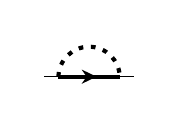
\begin{tikzpicture}[x=0.75pt,y=0.75pt,yscale=-0.65,xscale=0.65, baseline=(XXXX.south) ]
    \path (0,57);\path (87.33333587646484,0);\draw    ($(current bounding box.center)+(0,0.3em)$) node [anchor=south] (XXXX) {};
    %Straight Lines [id:da4779610823231175] 
    \draw [color={rgb, 255:red, 0; green, 0; blue, 0 }  ,draw opacity=1 ]   (12.33,36.33) -- (22.78,36.33) ;
    %Straight Lines [id:da9873503675232067] 
    \draw [color={rgb, 255:red, 0; green, 0; blue, 0 }  ,draw opacity=1 ]   (68.1,36.33) -- (78.55,36.33) ;
    %Straight Lines [id:da09313351721820862] 
    \draw [color={rgb, 255:red, 0; green, 0; blue, 0 }  ,draw opacity=1 ][line width=1.5]    (22.78,36.33) -- (68.1,36.33) ;
    \draw [shift={(51.04,36.33)}, rotate = 180] [fill={rgb, 255:red, 0; green, 0; blue, 0 }  ,fill opacity=1 ][line width=0.08]  [draw opacity=0] (11.07,-5.32) -- (0,0) -- (11.07,5.32) -- (7.35,0) -- cycle    ;
    %Shape: Arc [id:dp7767262671888671] 
    \draw  [draw opacity=0][dash pattern={on 1.69pt off 2.76pt}][line width=1.5]  (22.78,36.33) .. controls (23.05,23.96) and (33.2,14.05) .. (45.62,14.11) .. controls (58.08,14.17) and (68.16,24.25) .. (68.24,36.67) -- (45.51,36.84) -- cycle ; \draw  [color={rgb, 255:red, 0; green, 0; blue, 0 }  ,draw opacity=1 ][dash pattern={on 1.69pt off 2.76pt}][line width=1.5]  (22.78,36.33) .. controls (23.05,23.96) and (33.2,14.05) .. (45.62,14.11) .. controls (58.08,14.17) and (68.16,24.25) .. (68.24,36.67) ;  
    \end{tikzpicture}
\end{gathered}$.

\textbf{Assuming quasiparticles\dots} 
$\scriptstyle v(\vb*{q} + \vb*{G}) = \frac{4\pi }{V \abs*{\vb*{q} + \vb*{G}}^2}$.
$\scriptstyle \Sigma \stackrel{\int_{\text{contour}}}{=} \Sigma^{\text{COH}} + \Sigma^{\text{SEX}}$,
$\scriptstyle \epsilon_{\vb*{G} \vb*{G}'}(\vb*{q}, \omega) = \delta_{\vb*{G} \vb*{G}'} - v(q + \vb*{G}) \chi_{\vb*{G} \vb*{G}'}(\vb*{q}, \omega)$, 
$\scriptstyle M_{n n'}(\vb*{k}, \vb*{q}, \vb*{G}) = \mel*{n \vb*{k} + \vb*{q}}{\ee^{\ii (\vb*{q} + \vb*{G}) \cdot \vb*{r}}}{n' \vb*{k}}$
\begin{equation}
    \scriptsize
    \begin{aligned}
    \mel{n \vb*{k}}{\Sigma^{\text{SEX}}(\omega)}{n' \vb*{k}} 
    &= - \sum_{n''}^{\text{occ}} \sum_{\vb*{q} \vb*{G} \vb*{G}'}
    M^*_{n'' n} (\vb*{k}, - \vb*{q}, - \vb*{G}) M_{n'' n'} (\vb*{k}, - \vb*{q},  -\vb*{G}') \\
    &\quad\quad \times  \epsilon^{-1}_{\vb*{G} \vb*{G}'}(\vb*{q}, \omega - E_{n'', \vb*{k} - \vb*{q}}) 
    v(\vb*{q} + \vb*{G}') ,
    \end{aligned}
    \label{eq:sex}
\end{equation}
\begin{equation}
    \scriptsize
    \begin{aligned}
        \mel{n \vb*{k}}{\Sigma^{\text{COH}}(\omega)}{n' \vb*{k}} 
        &= \frac{\ii}{2\pi} \sum_{n''} \sum_{\vb*{q}, \vb*{G}, \vb*{G}'} 
        M^*_{n'' n} (\vb*{k}, - \vb*{q}, - \vb*{G})  M_{n'' n'} (\vb*{k}, - \vb*{q},  -\vb*{G}') \\
        & \times \int_{0}^{\infty} \dd{\omega'} 
        \frac{
            [\epsilon^{\text{r}}_{\vb*{G} \vb*{G}'}]^{-1} (\vb*{q}, \omega')
            - [\epsilon^{\text{a}}_{\vb*{G} \vb*{G}'}]^{-1} (\vb*{q}, \omega') 
        }{\omega - E_{n \vb*{k}} - \omega' + \ii 0^+ \sgn(E_{n \vb*{k}})} v(\vb*{q}+\vb*{G}') .
    \end{aligned}
    \label{eq:coh}
\end{equation}
\begin{equation}
    \scriptsize
    \begin{aligned}
        \chi^{\text{r/a}}_{\vb*{G} \vb*{G}'}(\vb*{q}, \omega)
        &= \sum_{\vb*{k}} \sum_{n}^{\text{occ}} \sum_{n'}^{\text{emp}} 
        M_{n n'} (\vb*{k}, \vb*{q}, \vb*{G}) M^*_{nn'} (\vb*{k}, \vb*{q}, \vb*{G}') \\
        &\times \left(
        \frac{
            1
        }{
            \omega + E_{n, \vb*{k} + \vb*{q}} - E_{n' \vb*{k}} \pm \ii 0^+
        }
        + \frac{
            1
        }{
            - \omega + E_{n, \vb*{k} + \vb*{q}} - E_{n' \vb*{k}} \mp \ii 0^+
        }
        \right).
    \end{aligned}
    \label{eq:chi}
\end{equation}

What a splendid equation system! 

\textbf{In practice\dots we always use GPP} $\epsilon(\omega)$ is assumed to be 
plasmon model-like, so -- we feed 
\begin{equation}
    \chi_{\vb*{G} \vb*{G}'}(\vb*{q}, \omega=0)
    = \sum_{\vb*{k}} \sum_{n}^{\text{occ}} \sum_{n'}^{\text{emp}} 
    M_{n n'} (\vb*{k}, \vb*{q}, \vb*{G}) M^*_{nn'} (\vb*{k}, \vb*{q}, \vb*{G}') 
    \frac{
        2
    }{
        E_{n, \vb*{k} + \vb*{q}} - E_{n' \vb*{k}} 
    }
\end{equation}
to \emph{analytic} expressions of $\Sigma^{\text{COH, SEX}}$.

\vspace{1cm}

\textbf{Huge simplification\dots} Hedin $\stackrel{\text{assuming $GW$}}{\rightarrow}$ 
$GW$ $\stackrel{\text{QP. approx.}}{\rightarrow}$ 
\eqref{eq:sex}, \eqref{eq:coh}, \eqref{eq:chi} $\stackrel{\text{GPP}}{\rightarrow}$ we are here

\textbf{But still burdensome} \emph{Summation over empty bands -- 1000-30000 bands!!!}

\end{frame}

\section{The mystery of \shortcode{pseudobands}}

\begin{frame}
\frametitle{The problem of summing over many empty bands}

\textbf{Empty states are important -- but why?}

\vspace{1cm}

\textbf{One further simplification trick:} \shortcode{pseudobands}. 
For $E_{n \vb*{k}} \gg E_{\text{F}}$:
\[
    \begin{aligned}
        \{ \phi_{n \vb*{k}} \}_{\text{adjacent energy block $n_{\text{b}}$}} 
        \rightarrow \sum_{n \in \text{block $n_{\text{b}}$}} \phi_{n \vb*{k}}, \\
        \{ E_{n \vb*{k}} \}_{\text{adjacent energy block $n_{\text{b}}$}} \rightarrow
        \frac{1}{\abs*{n_{\text{b}}}}  \sum_{n \in \text{block $n_{\text{b}}$}} E_{n \vb*{k}}.
    \end{aligned}
\]
4000 bands $\to$ $\sim 400$ to $\sim 1000$ bands.

\vspace{1cm}

\dots but is this snake oil? It makes no sense!!!

\end{frame}

\begin{frame}[allowframebreaks]
\frametitle{Understanding \shortcode{pseudobands}: energy averaging}

\textbf{Observation} 
\begin{itemize}
    \item $\chi \sim M M^* \times \text{some-function}(E_{\text{emp}} - E_{\text{occ}})$;
    \item $\Sigma^{\text{COH}} \sim M M^* \times \text{some-function}(\omega - E)$; 
    \item We are only interested in $\omega \sim E_{\text{F}}$.
\end{itemize}

\vspace{0.5cm}

\faHandPointRight For $E_{n \vb*{k}} \gg E_{\text{F}}$ ($\omega$):  
$\text{energy-dependent factors} \sim \const.$ for all $\vb*{k}$.

\vspace{0.5cm}

Thus for both $\chi$ and $\Sigma^{\text{COH}}$ involving summation over empty bands:
\begin{equation}
    \sum_{n''}^{\text{high emp. bands}} M_{n'' n}^* M_{n'' n'} \times \cdots 
    = \sum_{\text{block $n_{\text{b}}$}} \cdots \times \sum_{n'' \in \text{block $n_{\text{b}}$}}
    M_{n'' n}^* M_{n'' n'}.
\end{equation}
In RHS $E_{\text{emp}}$ is replaced by the average energy.

\framebreak

\begin{center}
    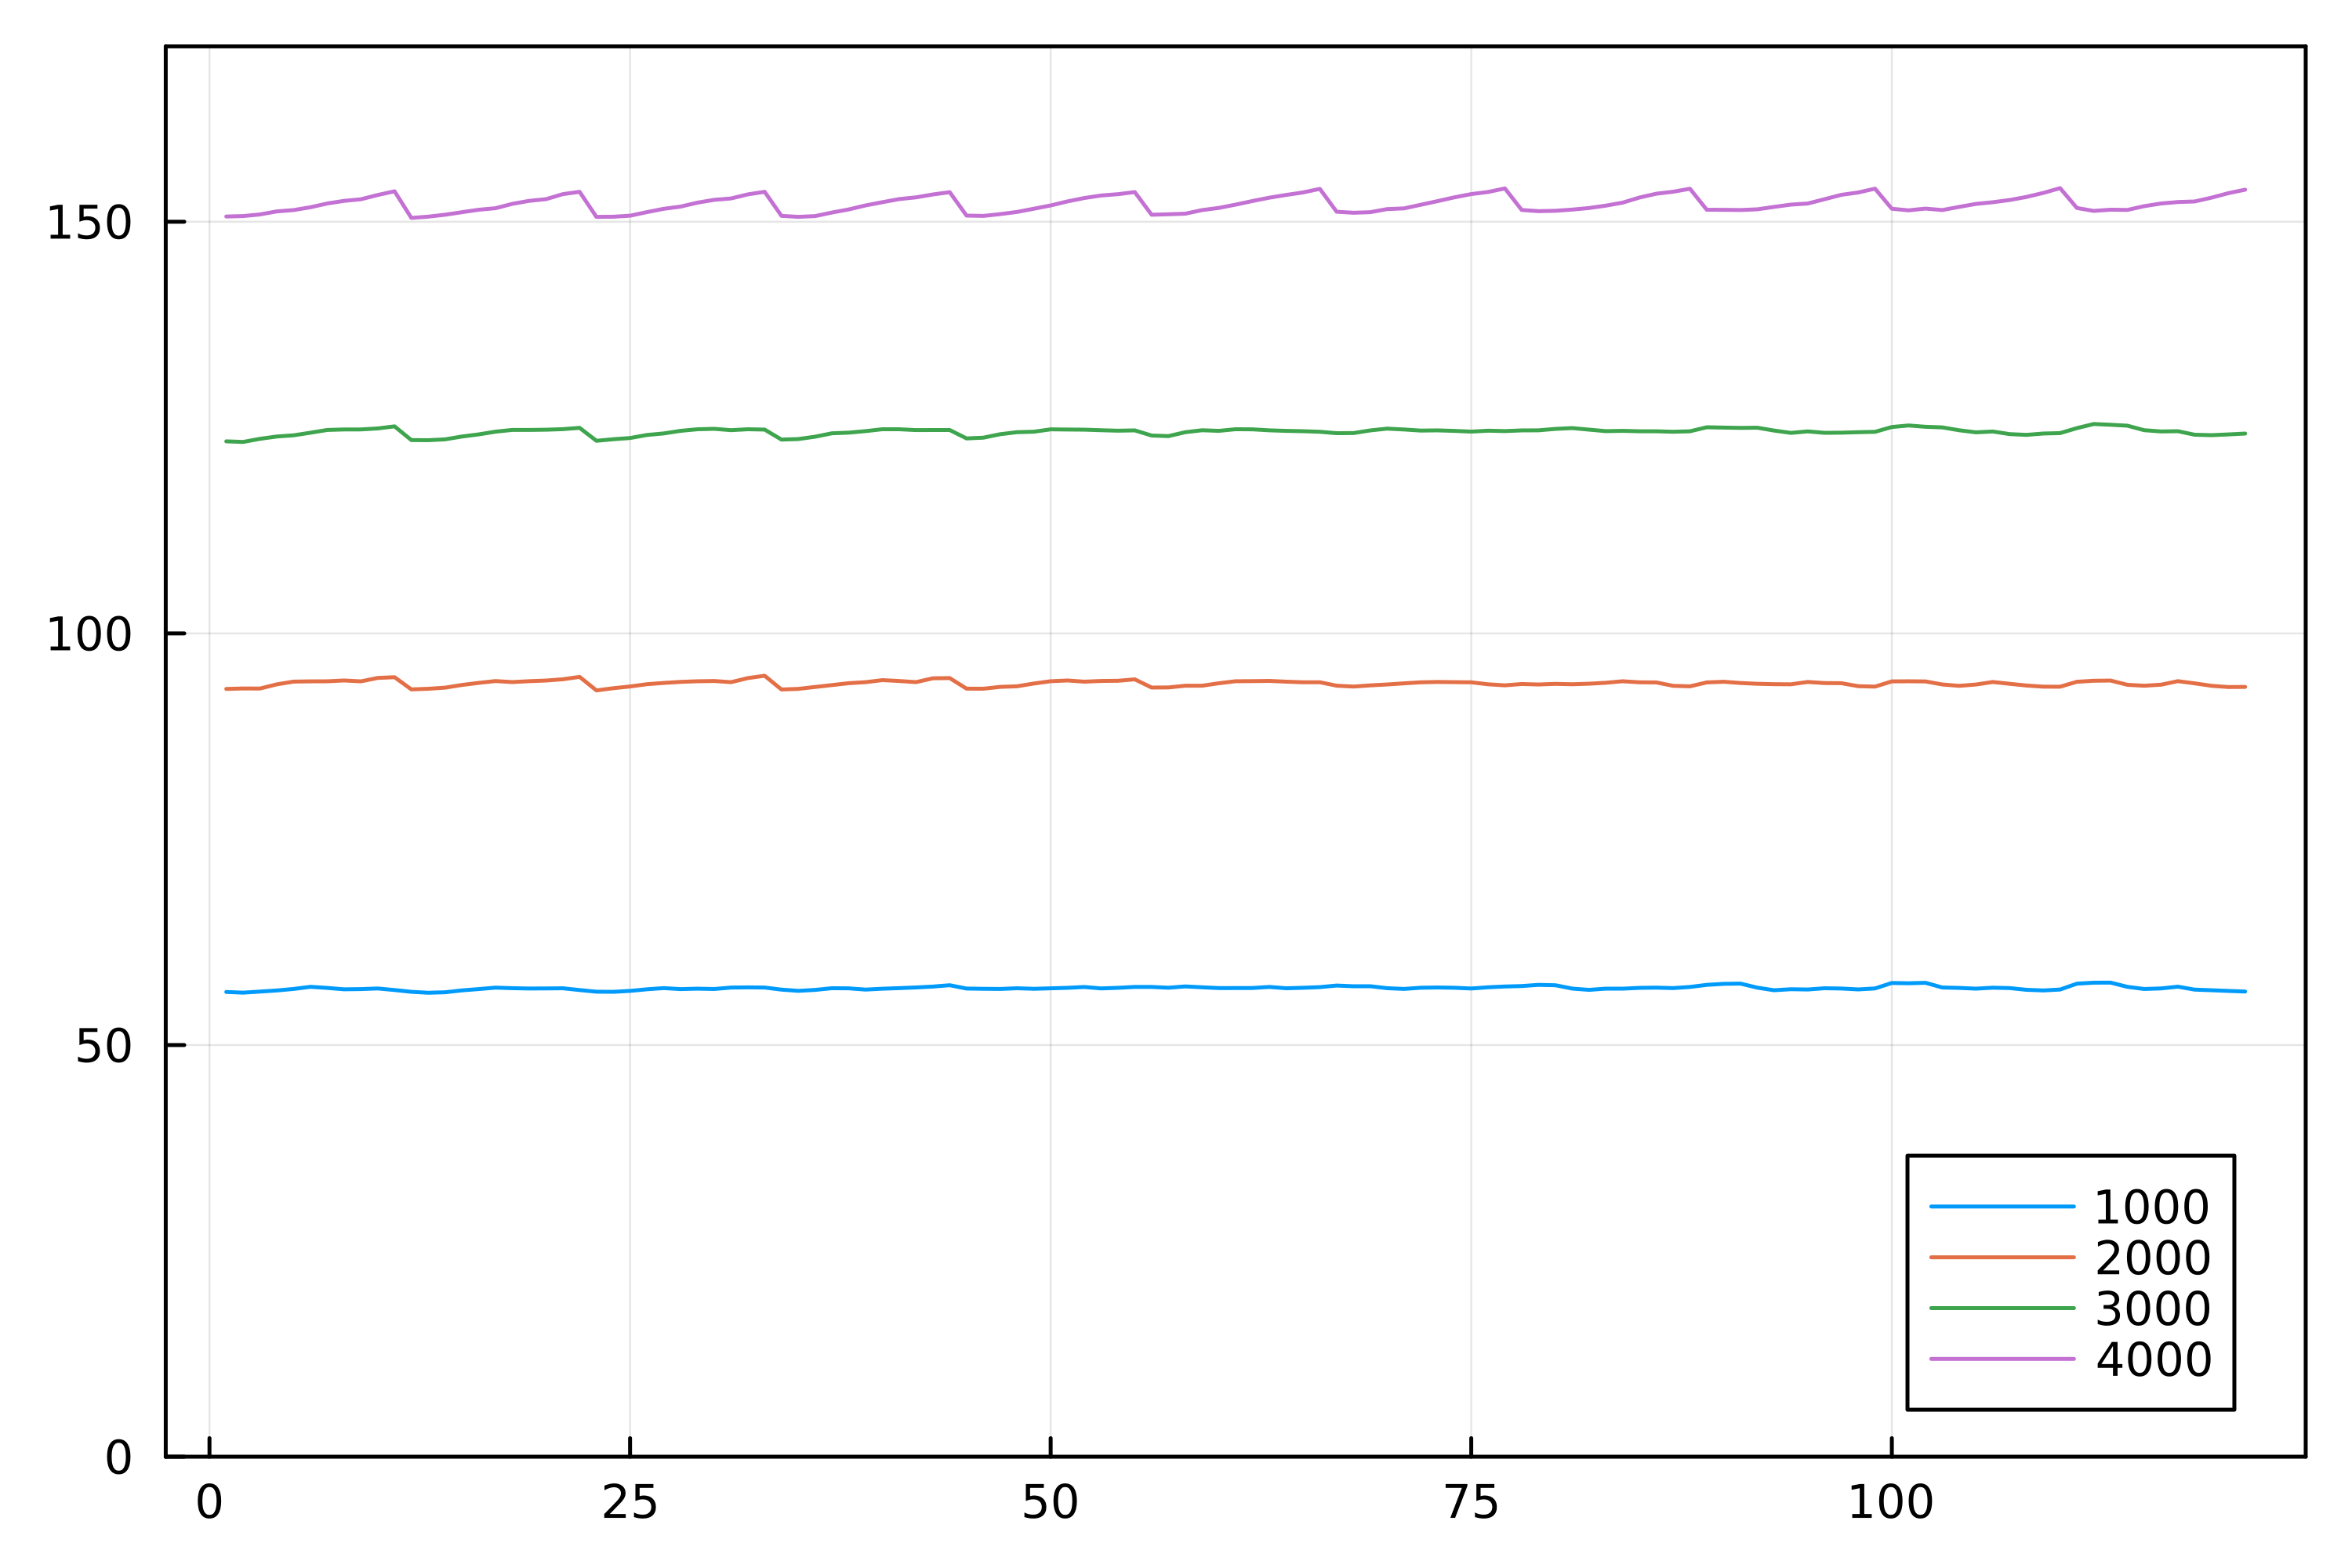
\includegraphics[width=0.45\textwidth]{../data/energy/energies-different-blocks.png}
    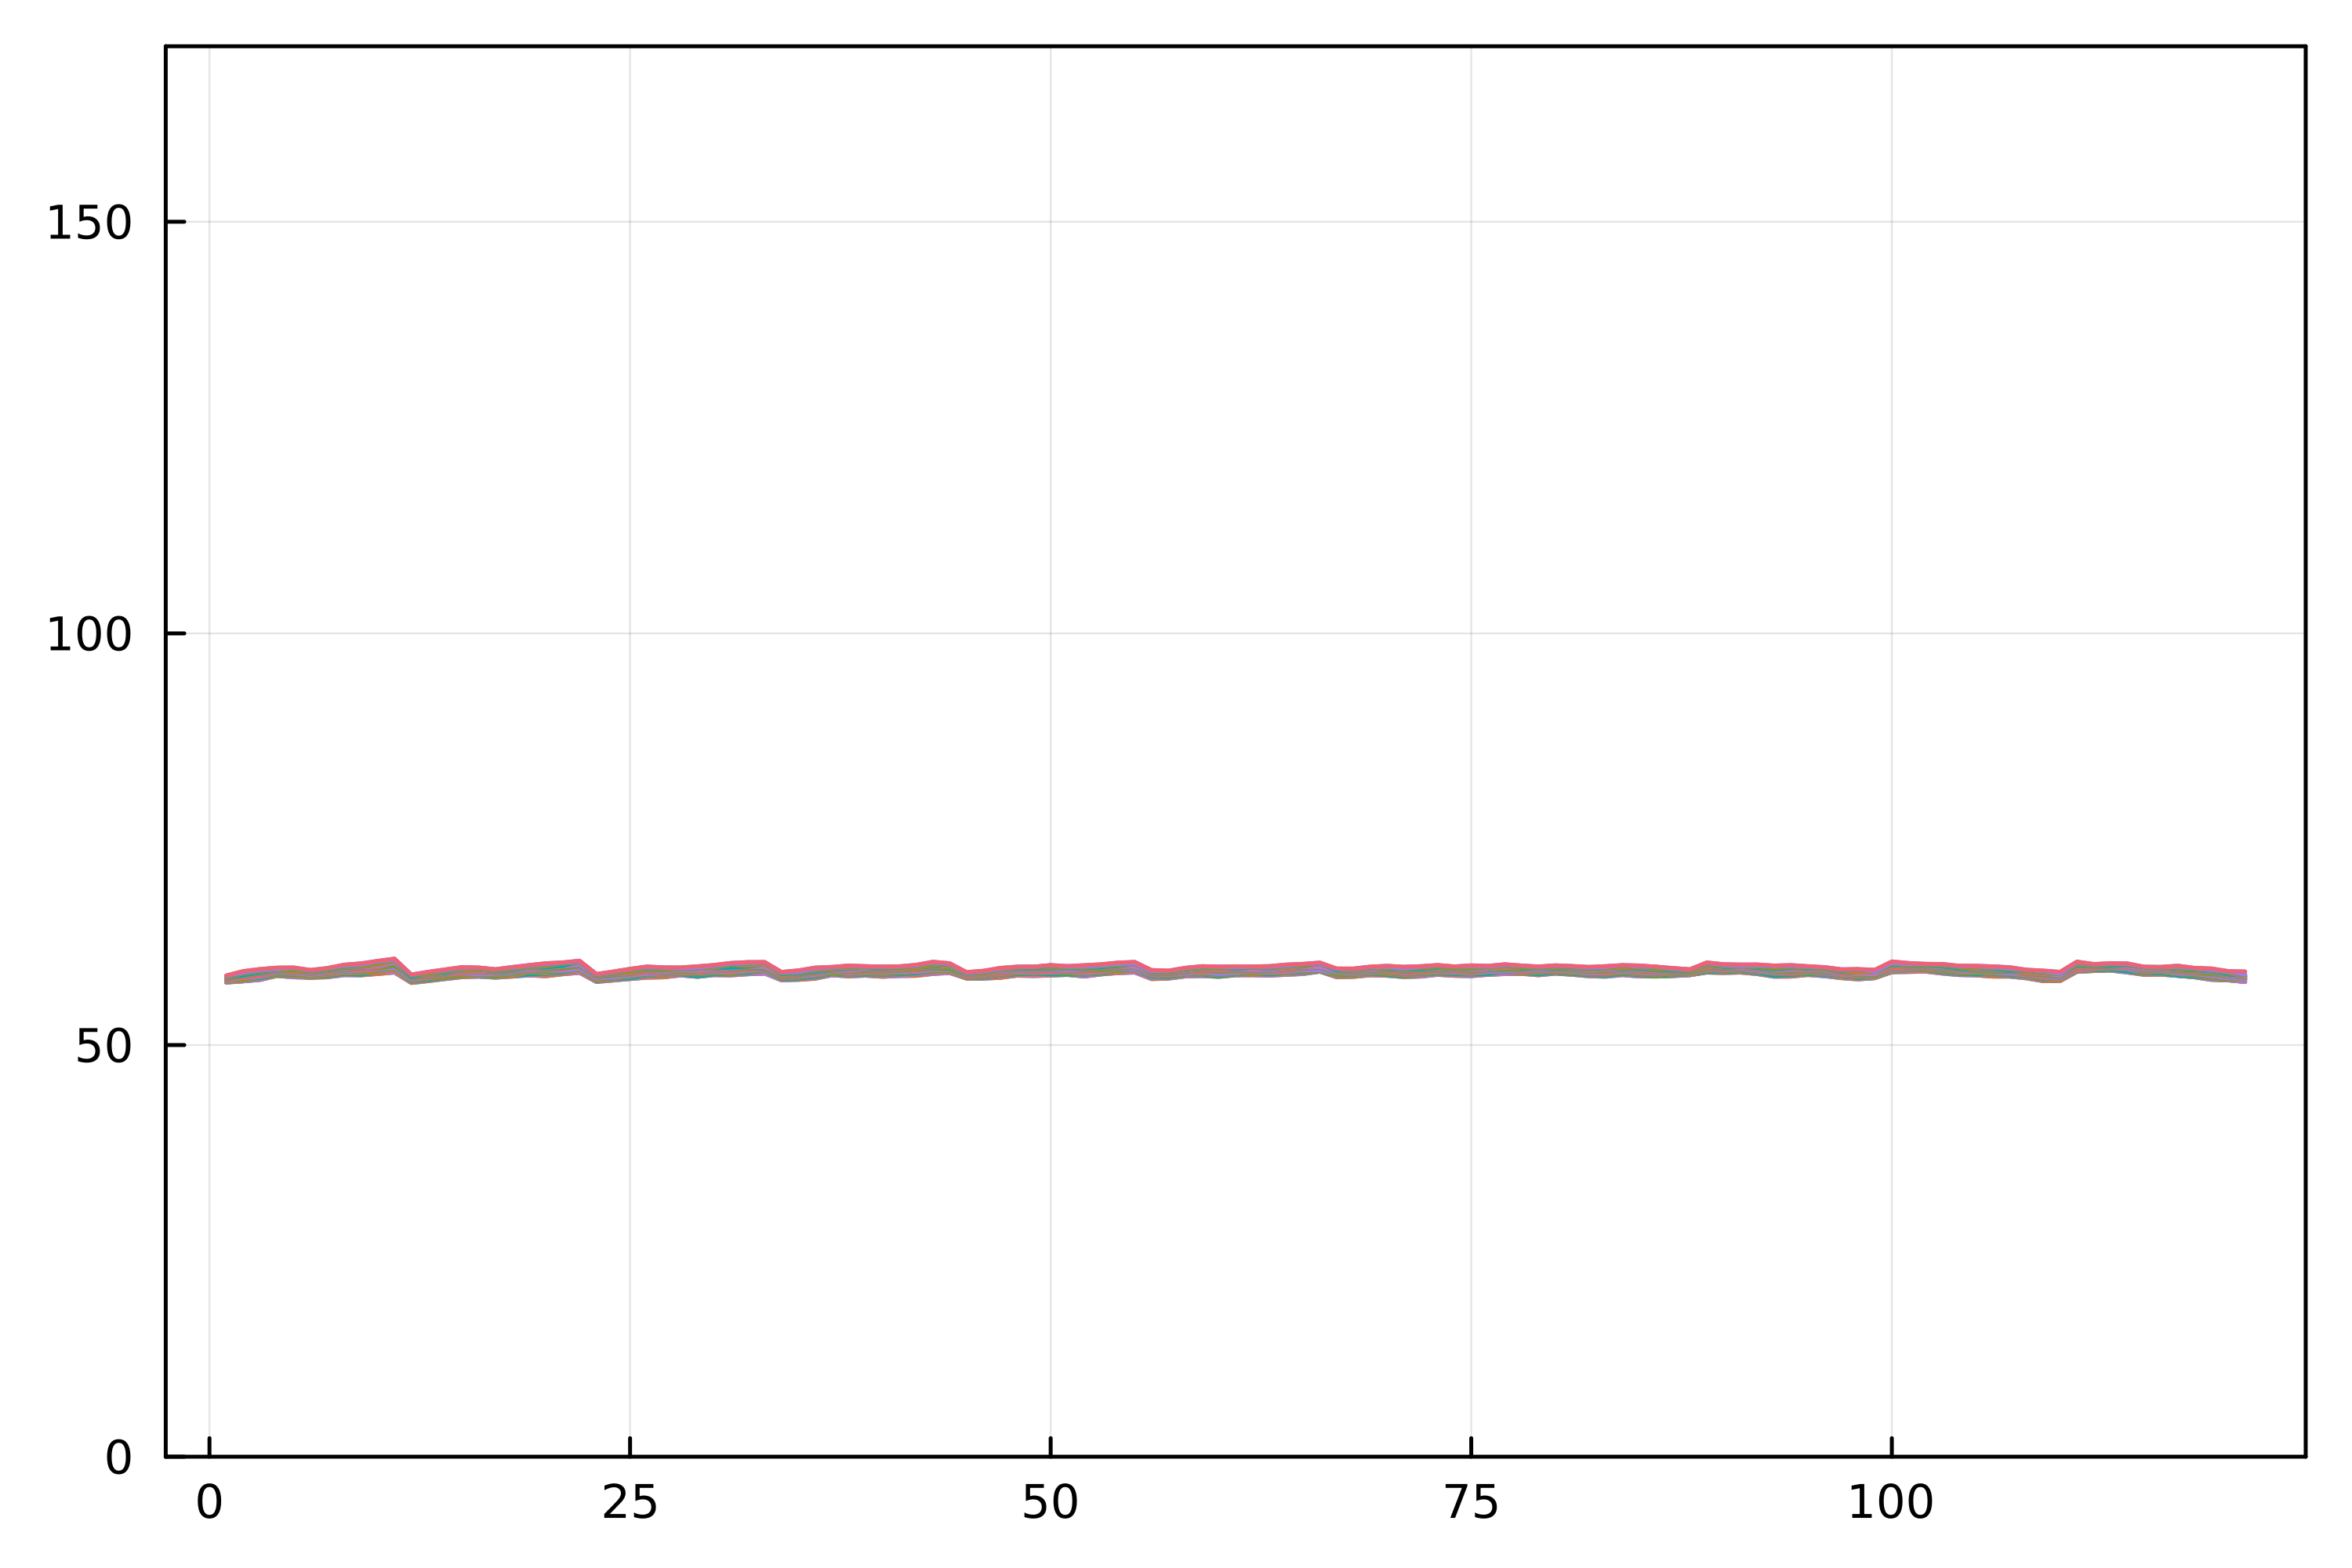
\includegraphics[width=0.45\textwidth]{../data/energy/energies-same-blocks-1062.png}
\end{center}

\textbf{Example} High-energy DFT bands of \ce{WTe2} monolayer 
(ONCV-SG15, 120 electrons; \SI{80}{Ry} cutoff, $20 \times 20 \times 1$ grid). 
$x$ axis = $\vb*{k}$ index in irreducible 1BZ; 
fastest varying coordinate = $k_y$ 

\vspace{0.5cm}

\begin{itemize}
    \item[\faHandPointRight] Bands above 1000 are generally flat (but dispersion $\uparrow$ as $n$ $\uparrow$)
    \item[\faHandPointRight] Low-lying pseudobands blocks are very close in energy 
    (but $1 / (E_{\text{emp}} - E_{\text{occ}})$ more sensitive to dispersion)
\end{itemize}

\framebreak

\begin{center}
    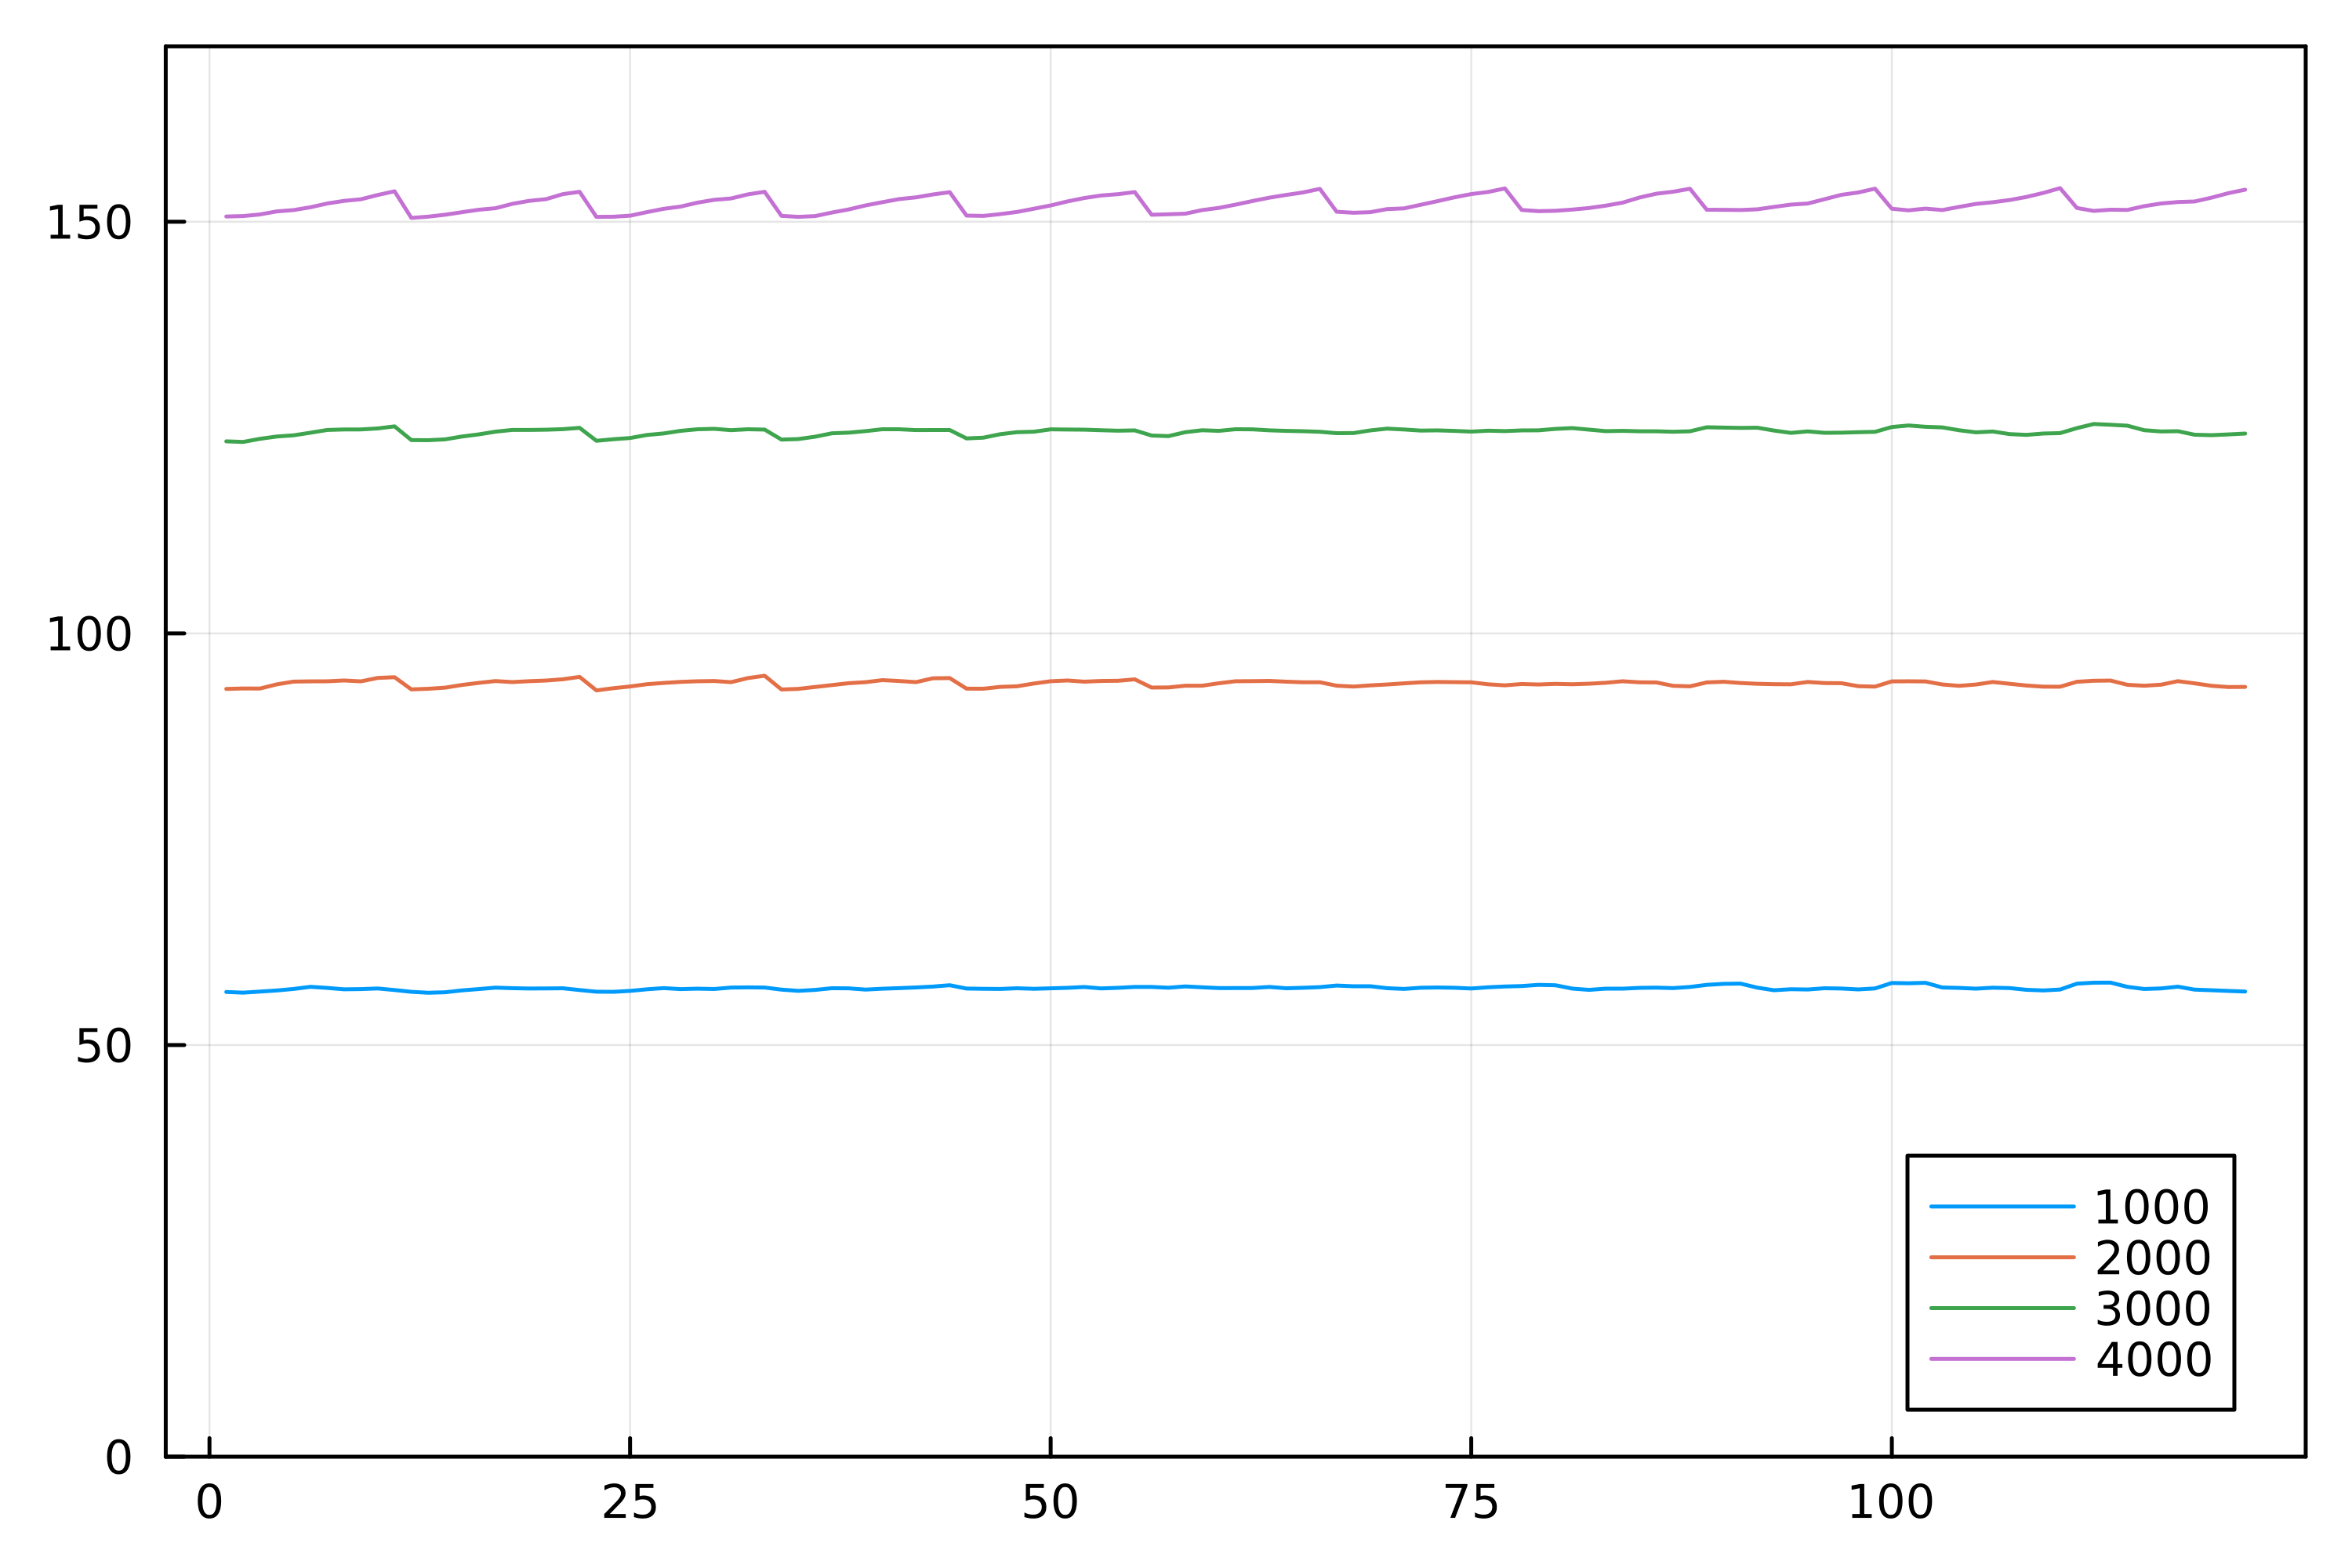
\includegraphics[width=0.45\textwidth]{../data/energy/energies-different-blocks.png}
    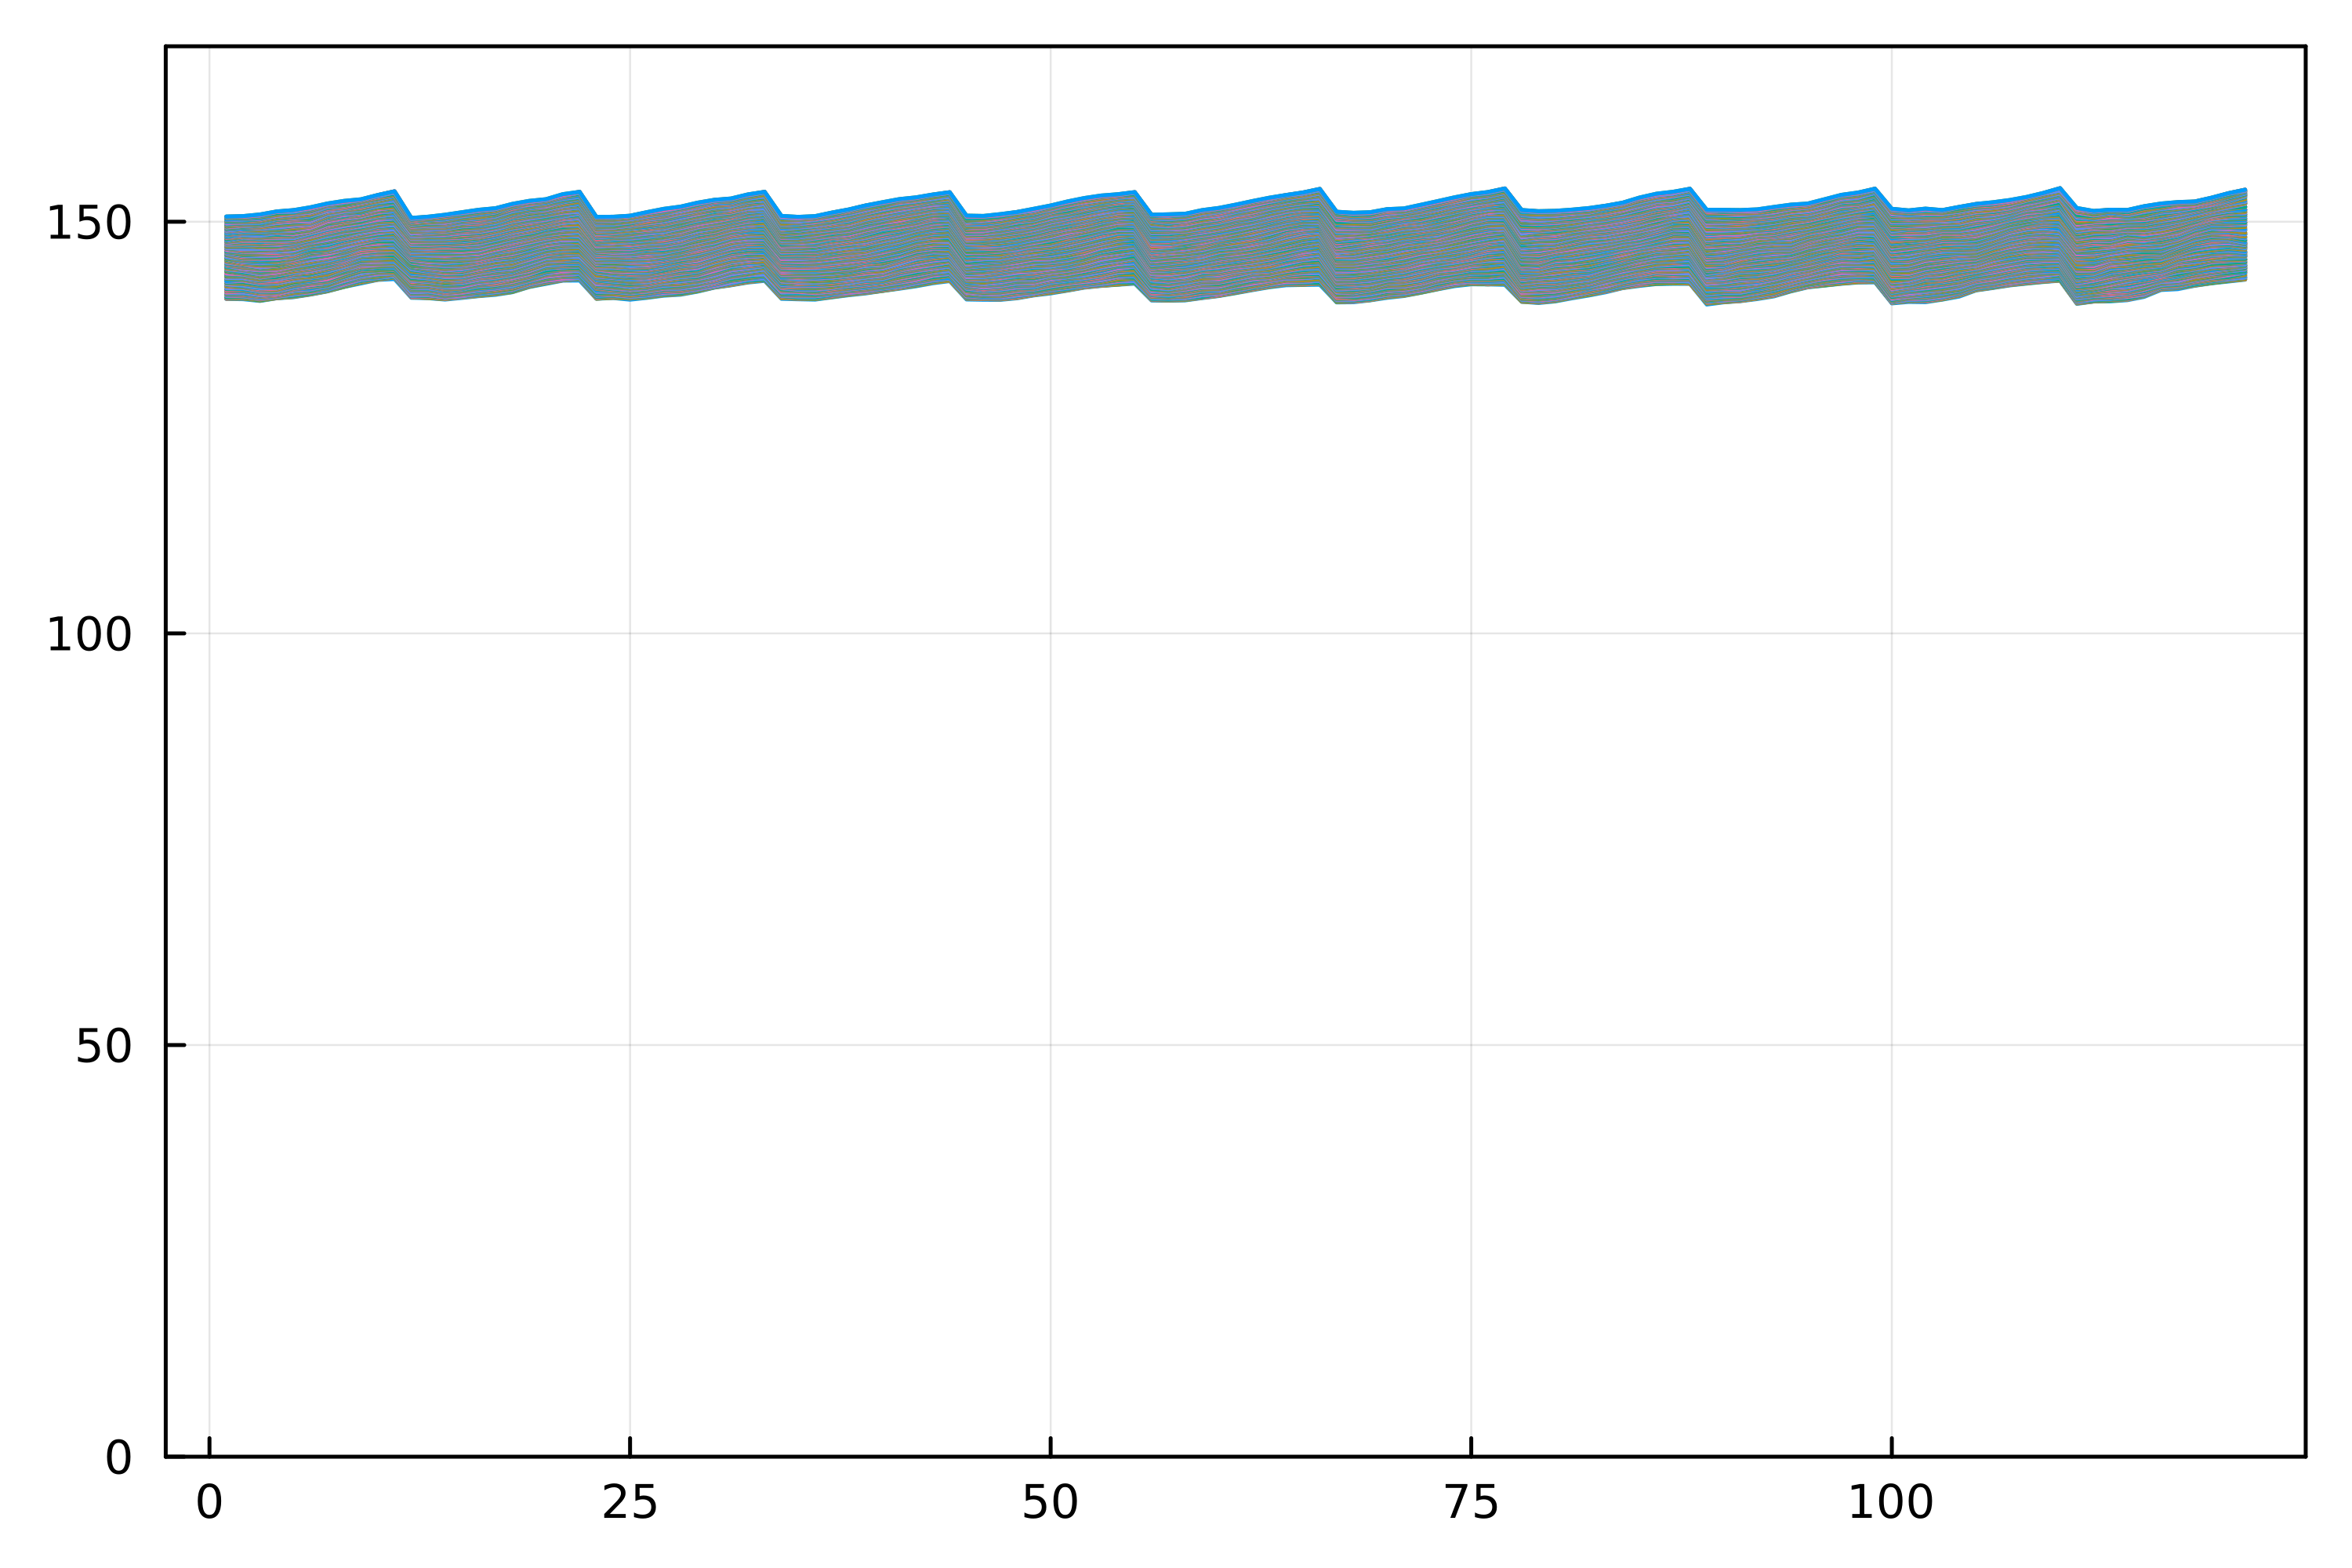
\includegraphics[width=0.45\textwidth]{../data/energy/energies-same-blocks-4000.png}
\end{center}

\textbf{Example} High-energy DFT bands of \ce{WTe2} monolayer 
(ONCV-SG15, 120 electrons; \SI{80}{Ry} cutoff, $20 \times 20 \times 1$ grid). 
$x$ axis = $\vb*{k}$ index in irreducible 1BZ; 
fastest varying coordinate = $k_y$ 

\vspace{0.5cm}

\begin{itemize}
    \item[\faHandPointRight] Bands above 1000 are generally flat (but dispersion $\uparrow$ as $n$ $\uparrow$)
    \item[\faHandPointRight] High-energy blocks are more dispersive 
    (but $1 / (E_{\text{emp}} - E_{\text{occ}})$ is smaller so no worry)
\end{itemize}

\end{frame}

\begin{frame}
\frametitle{Understanding \shortcode{pseudobands}: wave function averaging?}

For \shortcode{pseudobands} to work, we need 
\begin{equation}
    \begin{aligned}
        \sum_{n'' \in \text{block $n_{\text{b}}$}} M_{n'' n}^* M_{n'' n'} 
        &\sim M_{\text{averaged band}, n}^* M_{\text{averaged band}, n'} \\
        &= \sum_{n''_1, n''_2 \in \text{block $n_{\text{b}}$}} M_{n_1'' n'} M_{n_2'' n}^*.
    \end{aligned}
    \label{eq:pseudobands-correct}
\end{equation}

\textbf{The problem: it of course isn't the case in general.}
If $[M_{n_1'' n'} M_{n_2'' n}^*]_{n_1'' n_2''}$ is a random matrix: 
$\text{LHS}:\text{RHS} \approx 0.3$.

\vspace{0.5cm}

\textbf{The question:} \emph{Then in which case is \eqref{eq:pseudobands-correct} correct in some sense?} 

\end{frame}

\section{Technical issues in calculating $M_{nn'}(\vb*{k}, \vb*{q}, \vb*{G})$}

\begin{frame}
\frametitle{The structure of $\phi_{n \vb*{k}}$}

\textbf{Plane wave basis} In BerkeleyGW \shortcode{WFN.h5}, 
\begin{equation}
    \phi_{n \vb*{k}}(\vb*{r}, \sigma) = \frac{1}{\sqrt{V}} \sum_{\vb*{G}} \ee^{\ii (\vb*{k} + \vb*{G}) \cdot \vb*{r}} c_{n \vb*{k}, \vb*{G} \sigma}.
\end{equation}    
Thus 
\begin{equation}
    M_{nn'}(\vb*{k}, \vb*{q}, \vb*{G}) 
    = \mel*{n \vb*{k} + \vb*{q}}{\ee^{\ii (\vb*{q} + \vb*{G}) \cdot \vb*{r}}}{n' \vb*{k}} 
    = \sum_{\vb*{G}', \sigma} c^*_{n \vb*{k} + \vb*{q}, \vb*{G} + \vb*{G}' \sigma} c_{n \vb*{k}, \vb*{G}' \sigma}.
\end{equation}

\textbf{Cutoff} Each $\vb*{k}$ has its own $\vb*{G}$-grid ($\sim 30000$ vectors for \SI{80}{Ry}).

\end{frame}

\begin{frame}
\frametitle{Procedure}

\textbf{Input} 
\begin{itemize}
    \item indices of $\vb*{k}, \vb*{q}$ in $\vb*{k}$-grid; 
    \item index of $\vb*{G}$ in $\vb*{G}$-grid of $\vb*{k}$ 
    (expect a $\vb*{G}$ in $GW$ $\vb*{G}$-grid, 
    cutoff = say \SI{30}{Ry}, not \SI{80}{Ry});
    \item $n, n'$.
\end{itemize}

\textbf{Procedure}
\begin{enumerate}
    \item find index of $\vb*{k}$
    \item find index of $\vb*{G} + \vb*{G}'$ in $\vb*{G}$-grid of $\vb*{k} + \vb*{q}$,
    for each $\vb*{G}'$ in $\vb*{G}$-grid of $\vb*{k}$
    \item do summation $\sum_{\vb*{G}', \sigma} c^*_{n \vb*{k} + \vb*{q}, \vb*{G} + \vb*{G}' \sigma} c_{n \vb*{k}, \vb*{G}' \sigma}$.
\end{enumerate}    

\vspace{0.5cm}

\textbf{Performance} Main bottleneck: finding $\vb*{G} + \vb*{G}'$.
Using \shortcode{StaticArrays.jl} helps a lot! 

\end{frame}

\section{\shortcode{pseudobands} for $\chi$}

\begin{frame}
\frametitle{$\chi$ revisited}

Under GPP:
\begin{equation}
    \begin{aligned}
        \chi_{\vb*{G} \vb*{G}'}(\vb*{q}, \omega)^{\text{high band terms}}
        \approx \sum_{\vb*{k}} \sum_{\text{block $n_{\text{b}}$}}^{\text{emp}} 
        \frac{
            2
        }{
            E_{n, \vb*{k} + \vb*{q}} - E_{\text{average in block $n_{\text{b}}$}} 
        } \\
        \times \sum_{n' \in \text{block $n_{\text{b}}$}} \sum_{n}^{\text{occ}} 
        M_{n n'} (\vb*{k}, \vb*{q}, \vb*{G}) M^*_{nn'} (\vb*{k}, \vb*{q}, \vb*{G}') 
    \end{aligned}
\end{equation}

\vspace{0.5cm}

\textbf{Our goal} \emph{Finding how diagonal is}
\begin{equation}
    \sum_{n}^{\text{occ}} 
        M_{n n'} (\vb*{k}, \vb*{q}, \vb*{G}) M^*_{nn'} (\vb*{k}, \vb*{q}, \vb*{G}') 
\end{equation}

\end{frame}

\begin{frame}[allowframebreaks]
\frametitle{Numerical charaterization of 
$\scriptstyle \sum_{n}^{\text{occ}} M_{n n'} (\vb*{k}, \vb*{q}, \vb*{G}) M^*_{nn'} (\vb*{k}, \vb*{q}, \vb*{G}') $}

\textbf{Case 1: $\vb*{G} = \vb*{G}'$}  In this case $\scriptstyle \sum_{n}^{\text{occ}} M_{n n'} (\vb*{k}, \vb*{q}, \vb*{G}) M^*_{nn'} (\vb*{k}, \vb*{q}, \vb*{G}')$ is large and fairly diagonal

\begin{center}
    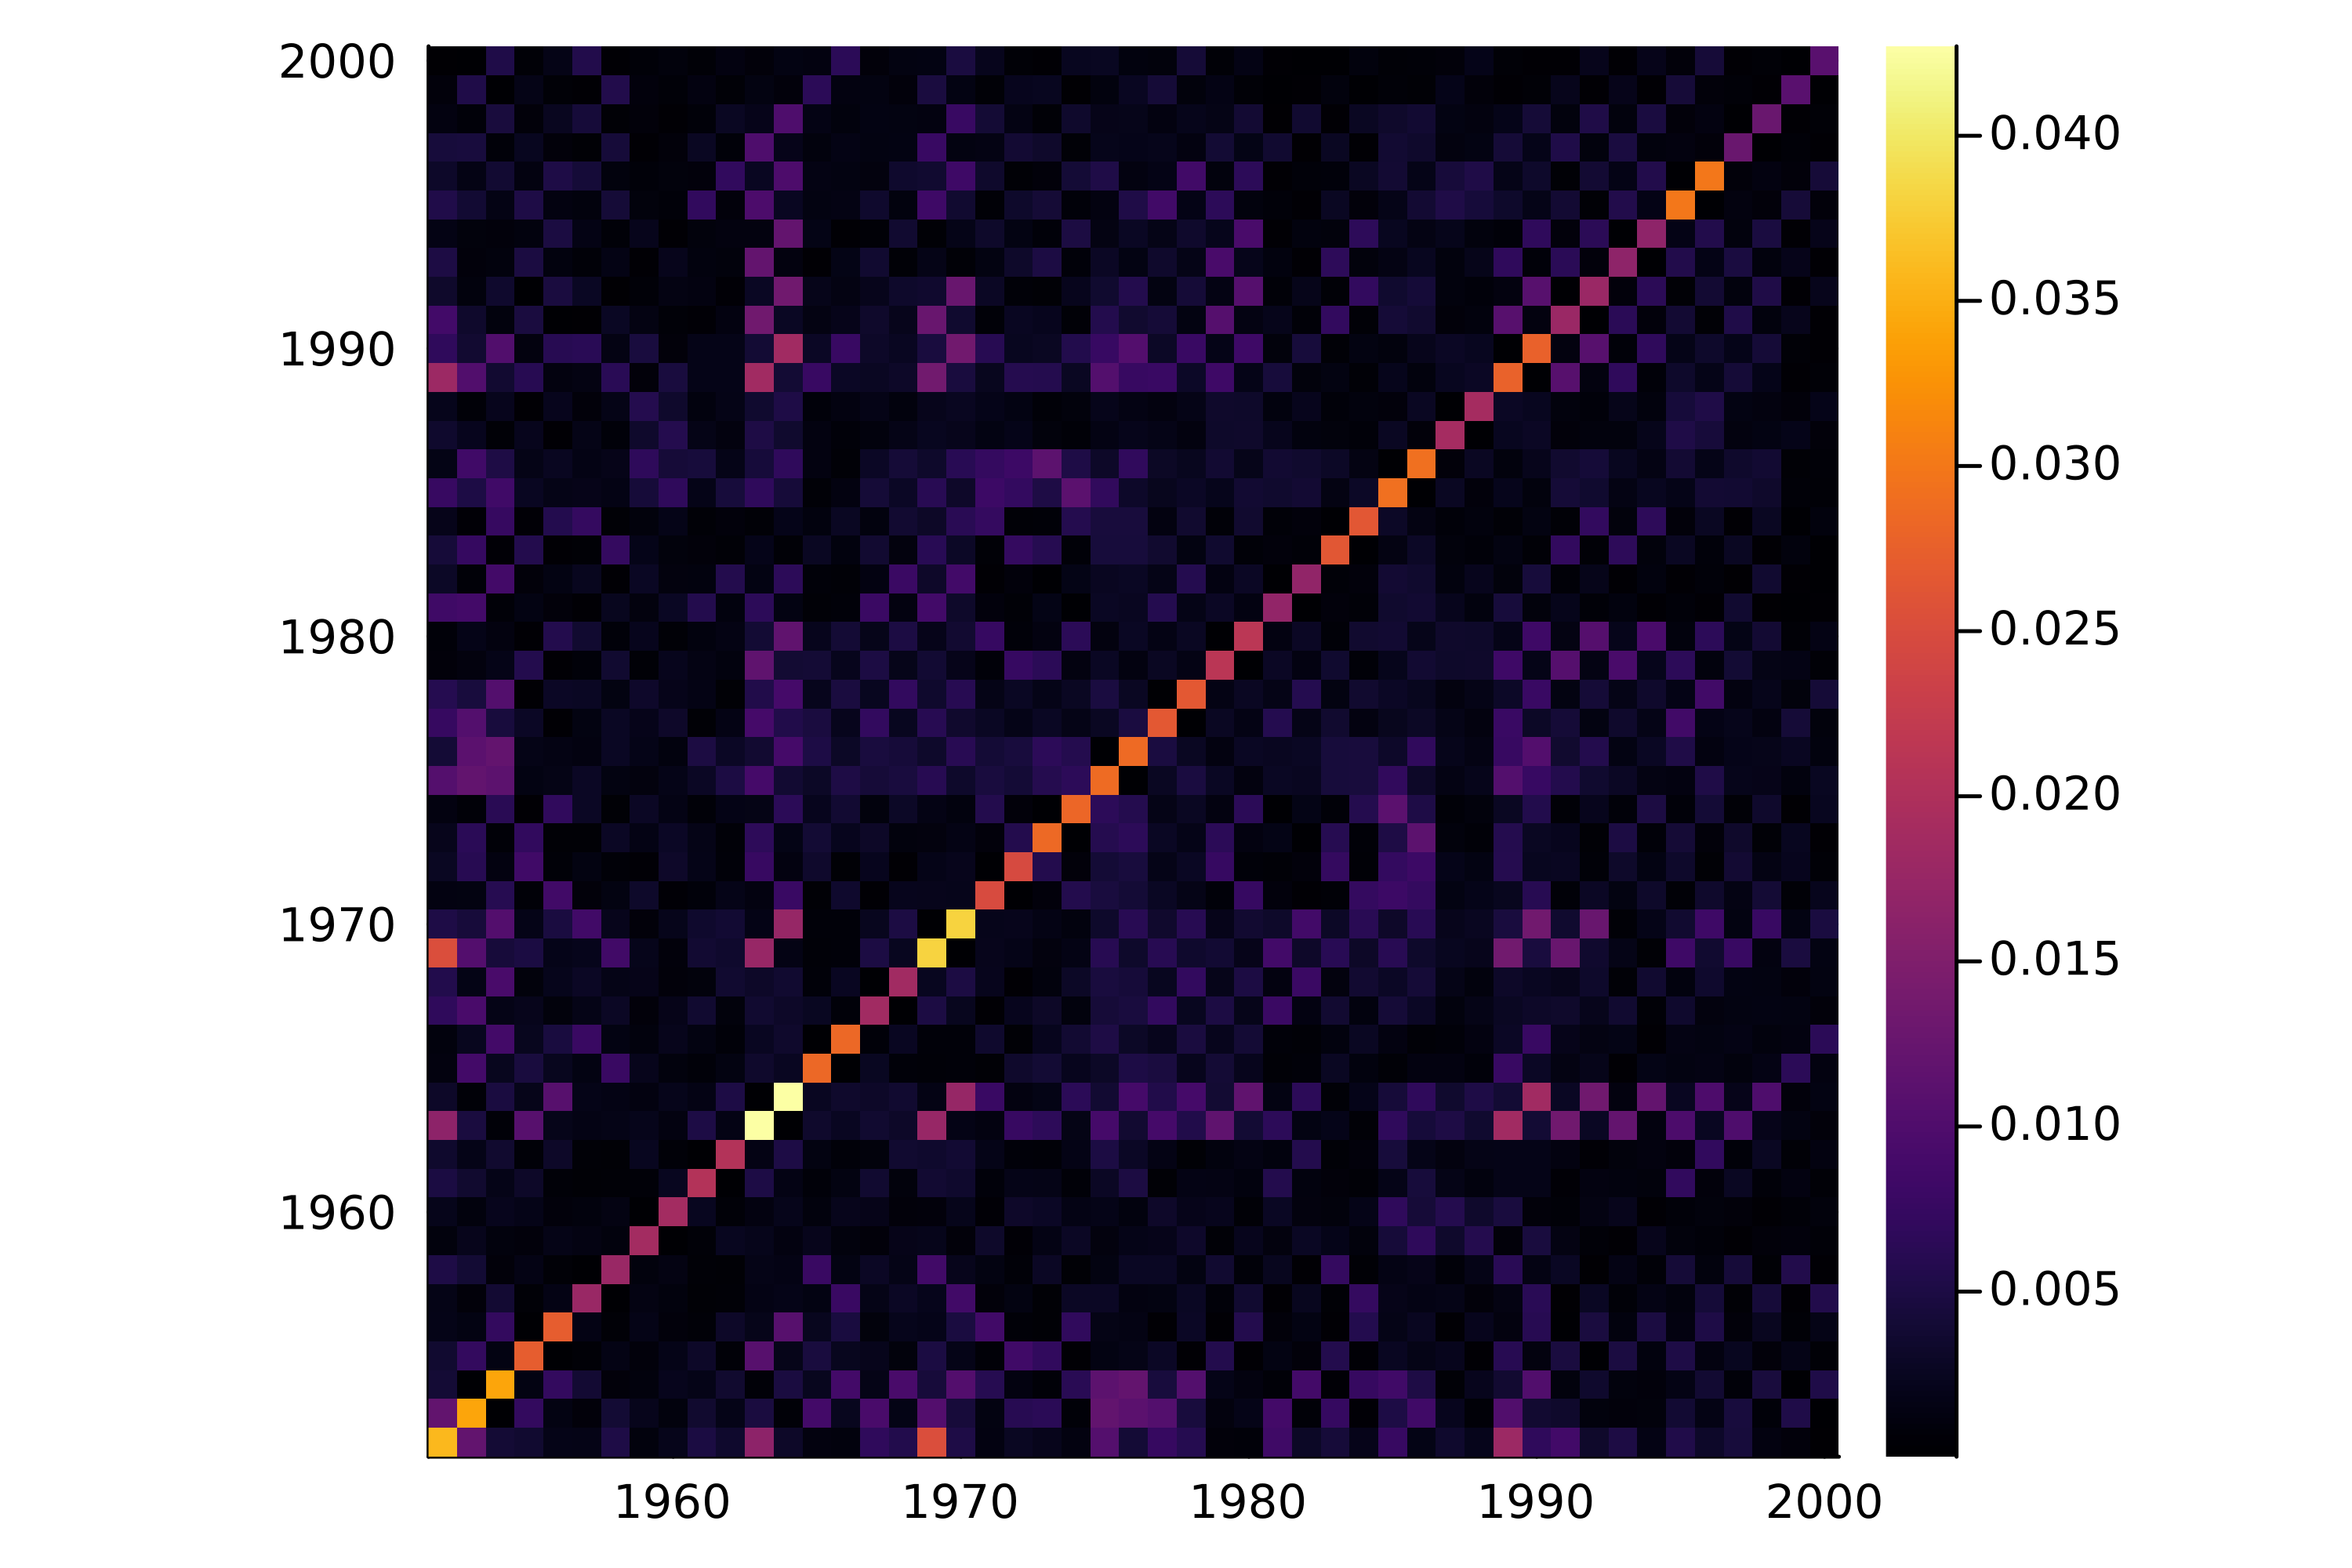
\includegraphics[width=0.6\textwidth]{../data/chi/nc_range-1951-2000-k_idx-1-q_idx-1-G_idx-810.png}
\end{center}

\textbf{Parameters} $\vb*{G} = (0, 1, -14), \vb*{k} = \vb*{k}_2 = (0, 0.00, 0), \vb*{q} = (0, 0.00, 0)$

\framebreak

\textbf{Case 1: $\vb*{G} = \vb*{G}'$}  In this case $\scriptstyle \sum_{n}^{\text{occ}} M_{n n'} (\vb*{k}, \vb*{q}, \vb*{G}) M^*_{nn'} (\vb*{k}, \vb*{q}, \vb*{G}')$ is large and fairly diagonal

\begin{center}
    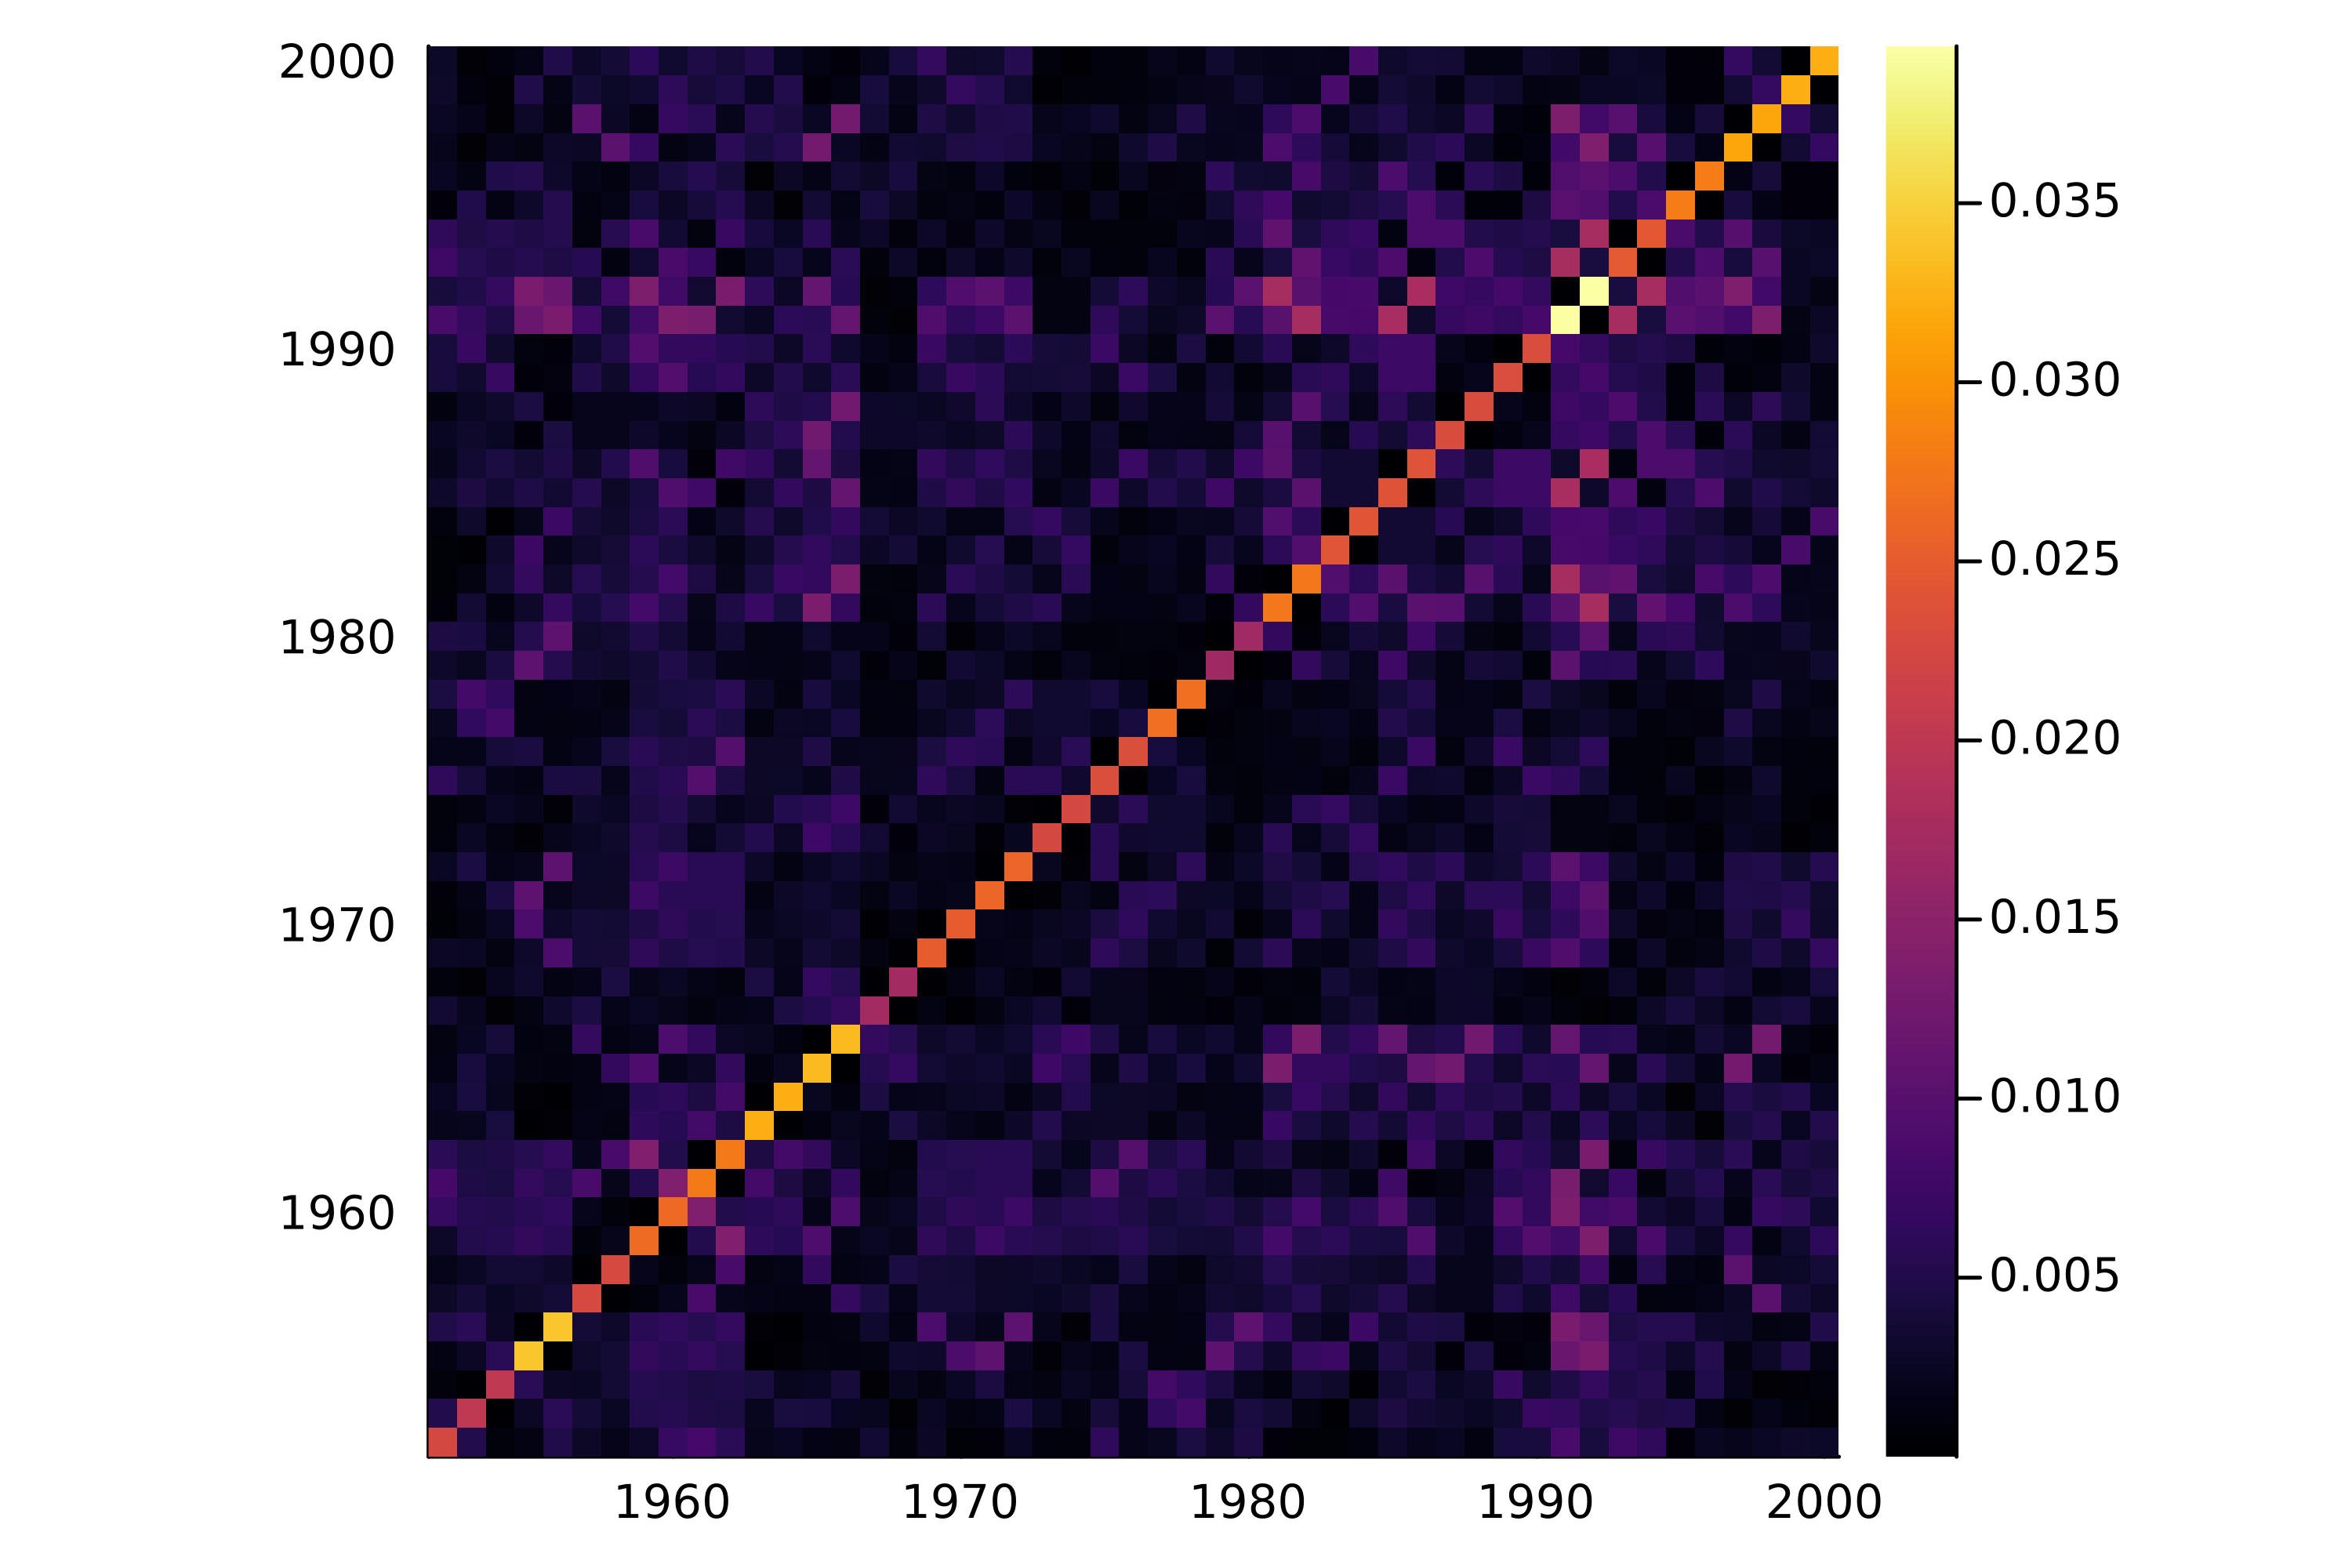
\includegraphics[width=0.6\textwidth]{../data/chi/nc_range-1951-2000-k_idx-2-q_idx-3-G_idx-810.png}
\end{center}

\textbf{Parameters} $\vb*{G} = (0, 1, -14), \vb*{k} = \vb*{k}_2 = (0, 0.05, 0), \vb*{q} = (0, 0.10, 0)$

\framebreak

\textbf{Case 1: $\vb*{G} = \vb*{G}'$}  In this case $\scriptstyle \sum_{n}^{\text{occ}} M_{n n'} (\vb*{k}, \vb*{q}, \vb*{G}) M^*_{nn'} (\vb*{k}, \vb*{q}, \vb*{G}')$ is large and fairly diagonal

\begin{center}
    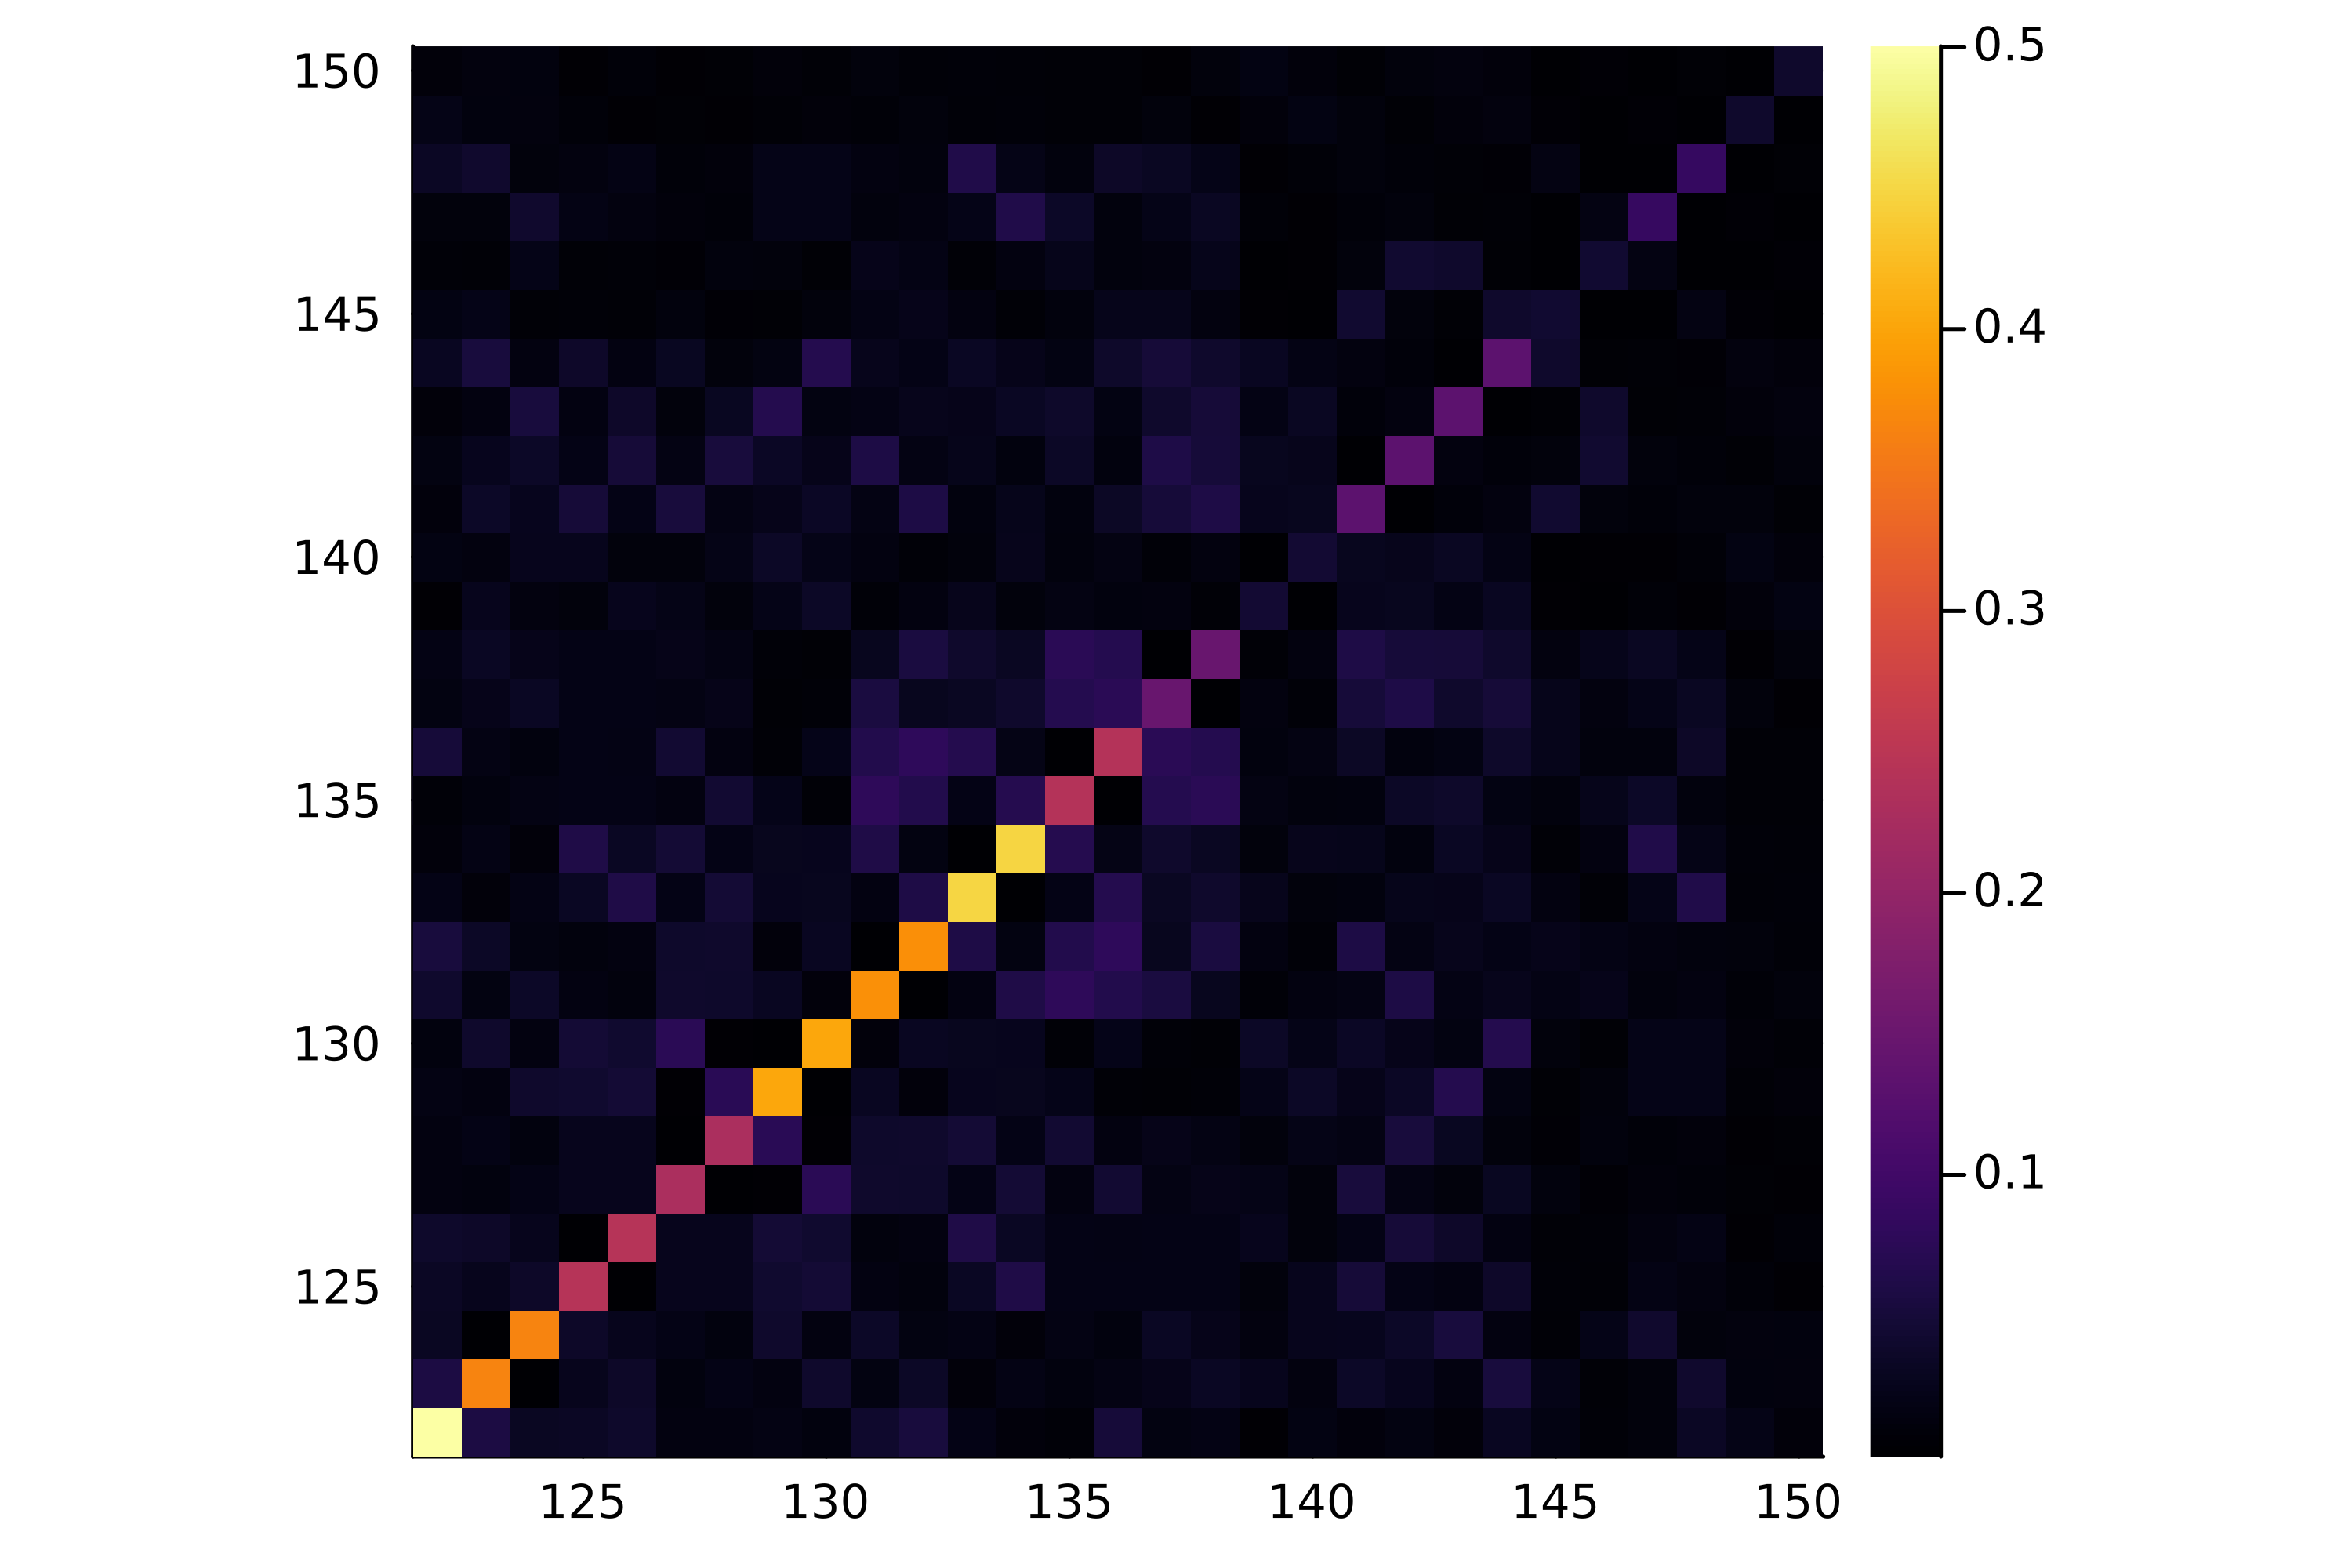
\includegraphics[width=0.6\textwidth]{../data/chi/nc_range-121-150-k_idx-2-q_idx-3-G_idx-100.png}
\end{center}

Strikingly, $\scriptstyle \sum_{n}^{\text{occ}} M_{n n'} (\vb*{k}, \vb*{q}, \vb*{G}) M^*_{nn'} (\vb*{k}, \vb*{q}, \vb*{G}')$ is still very diagonal for bands near Fermi surface!

\framebreak

\textbf{Case 2: $\vb*{G} \neq \vb*{G}'$} $\scriptstyle \sum_{n}^{\text{occ}} M_{n n'} (\vb*{k}, \vb*{q}, \vb*{G}) M^*_{nn'} (\vb*{k}, \vb*{q}, \vb*{G}')$ is very non-diagonal, 
but since the terms's random phases cancel each other so it's small

\begin{center}
    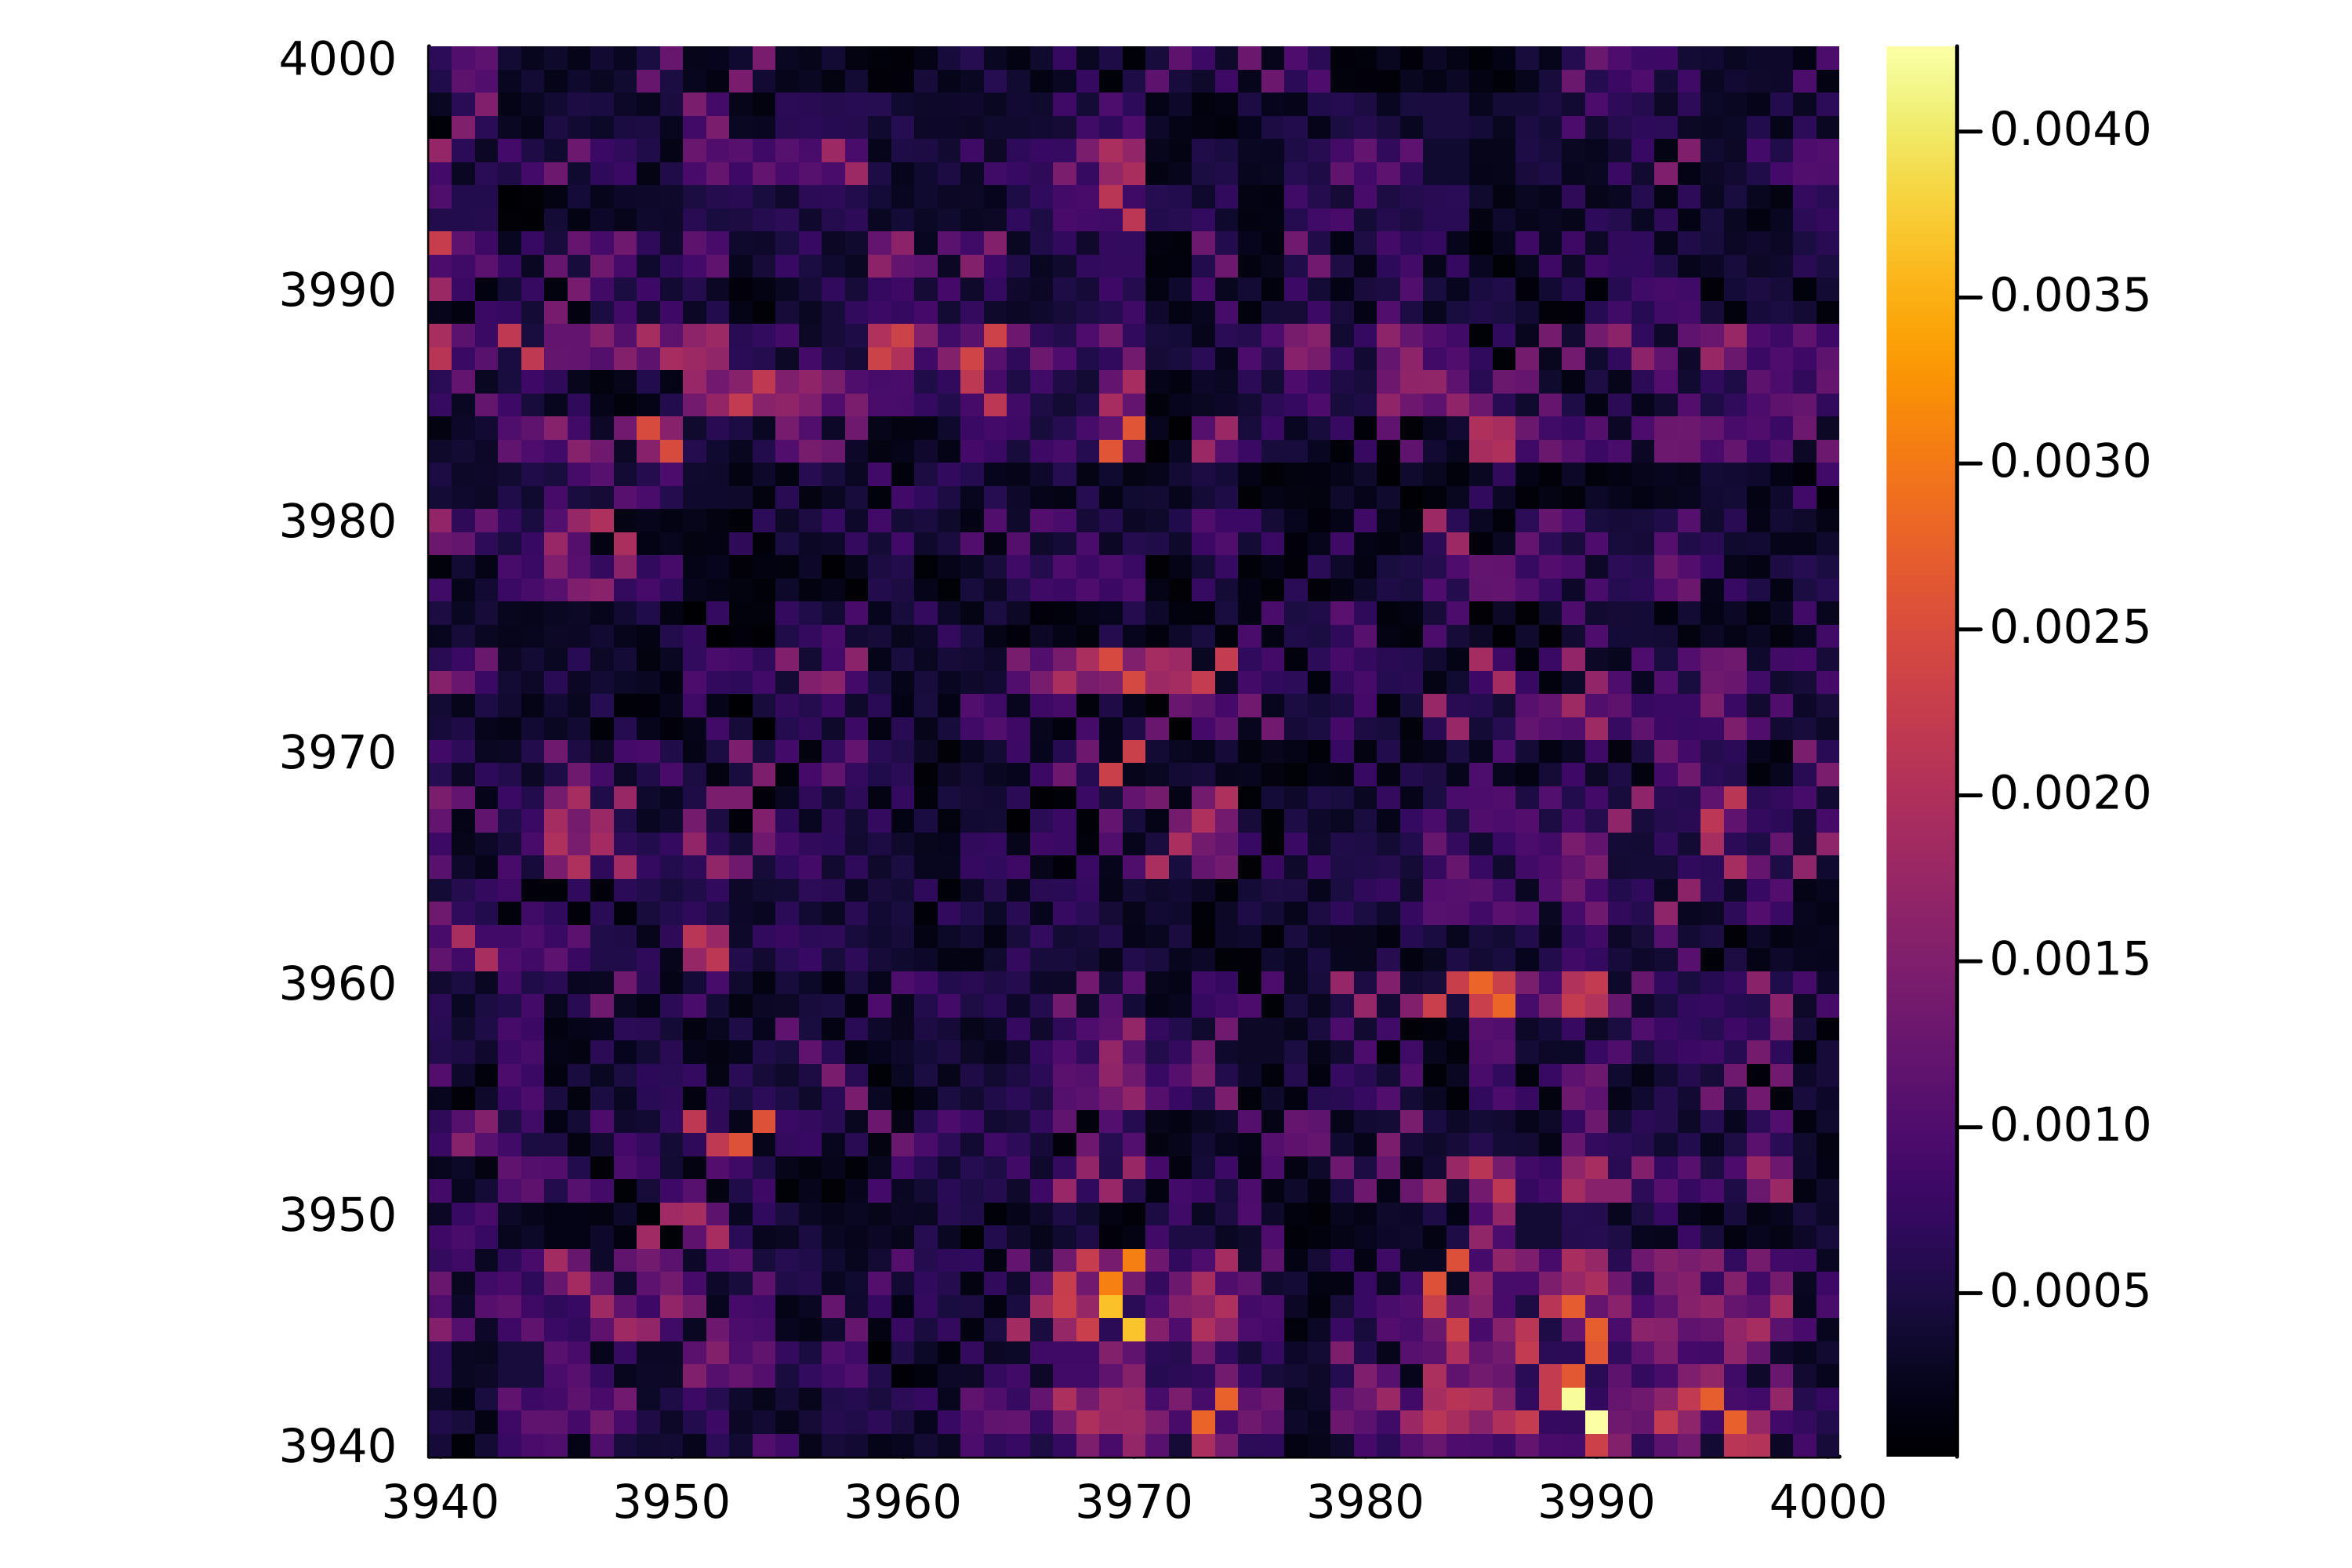
\includegraphics[width=0.6\textwidth]{../data/chi/nc_range-3939-4000-k_idx-2-q_idx-3-G1_idx-2000-G2_idx-2001.png}
\end{center}

\end{frame}

\begin{frame}
\frametitle{Half-way generalization about \shortcode{pseudobands} in $\chi$}

\begin{itemize}
    \item[\faHandPointRight] \shortcode{pseudobands} works  
    when it's necessary to do so 
    \item[\faHandPointRight] What prevents \shortcode{pseudobands} from working 
    around Fermi surface is the energy dispersion
\end{itemize}

\vspace{0.5cm}

\dots but do we have any theoretical explanation for this?

\end{frame}

\end{document}